\chapter{The LHC and CMS Detector} % (fold)
\label{cha:the_lhc_and_cms_machine}

In this chapter, the working and the design parameters of the Large Hadron Collider (LHC) and one of its general purpose detector, Compact Muon Solenoid (CMS), are briefly described.


%%%%%%%%%%%%%%%%%%%%%%%%%%%%%%%%%%%%%%%%%%%%%%%%%%%%%%%%%%%%%%%%%%
\section{The Large Hadron Collider} % (fold)
\label{sec:the_large_hadron_collider}

The famous quote ``{\textit{history repeats itself}}" applies well to the High Energy Physics (HEP) experiments. 
The starting point of experimental particle physics was the Rutherford $\alpha$-particle scattering, which was proposed by Ernest Rutherford and carried out by his two assistants - Hans Geiger and Ernest Marsden - in the early $20^{th}$ century~\cite{Hauptman2010}. 
In this experiment, a beam of $\alpha$-particles was fired at a thin gold foil and its scattering was observed on the photographic screen. 
Based on their experimental findings, they suggested the structure of the atom as we know it today, in which most of the mass is centred at the core of the atom known as the nucleus, and electrons  revolve around it. 
One hundred years after this classic experiment, the same techniques are employed today to explore the most basic constituents of the matter. 
Only, the technique changed from ``{\textit{natural accelerator}}"\footnote{radioactivity and cosmic rays} to the ``{\textit{man-made}}" accelerator.
The man made accelerator, also known as particle accelerator, can accelerate particles with speed close to the speed of light. 
The design and working of the particle accelerator has changed a lot over the period of time in going from eV to GeV and now to TeV range. 
Nowadays, accelerators are not only used in HEP experiments, but also extend their arenas to medical sciences such as production of radioisotopes for cancer treatments, 3-D X-rays, etc. and to the industrial applications involving material processing, sterilization, security scan, water treatment, and many more~\cite{Demarteau2016}. 

The Large Hadron Collider (LHC) is one such accelerator, and as the name suggests, it is  a hadron collider which can accelerate two proton beams, moving in opposite direction, to a maximum of 14 TeV center of mass energy in a 26.7 km long tunnel which is about 100 m underground spanning border areas of France and Switzerland. The LHC is the latest and the most-powerful particle accelerator and collider is built to improve our understanding of fundamental physics. It started its operation on 21$^{st}$ October 2008 and is housed in the tunnel previously used by Large Electron Positron (LEP) Collider. The European Organization for Nuclear Research (CERN) decided to switch this to hadron collider because of the following advantages:
\begin{itemize}
    \item A hadron collider can reach higher centre of mass energy because of very low synchrotron radiation\footnote{The radiation emitted by a charged particle during acceleration in a circular path is known as synchrotron radiation. As particles lose energy in emission of this radiation, an additional energy must be provided to keep the beam at constant energy.} emitted by hadrons as compared to electrons. Synchrotron radiation loss is directly proportional to $(Energy/mass)^4$.
    \item As hadrons are composite particles, they allow the possibility to scan over wider range of energies.
\end{itemize}
All particle accelerators have three major components:
\begin{itemize}
  \item Beam pipes
  \item Accelerating structure
  \item Magnet system
\end{itemize}
These components are explained briefly in the following sub-sections for the LHC.

%%%%%%%%%%%%%%%%%%%%%%%%%%%%%%%%%%%%%%%%%%%%%%%%%%%%%%%%%%%%%%%%%%
%%%%%%%%%%%%%%%%%%%%%%%%%%%%%%%%%%%%%%%%%%%%%%%%%%%%%%%%%%%%%%%%%%
\subsection{Beam Pipes} % (fold)
\label{sub:beam_pipes}

At the LHC, there are two beam pipes - each having a diameter of $\approx$ 6.3 cm in which proton beams travel in opposite directions. To avoid beam instability and loss of beam particles due to collision with gas molecules the beam pipes are kept at ultra-high vacuum\footnote{At LHC, three different vacuum systems are used. First one is used for beam pipe; second one for insulating the cryogenically cooled magnets and third one is used for insulating the helium distribution. In the latter two it just acts as a thermal insulator as the cryogenic parts are kept at 1.9 K ($\ang{-271.3}C$)} maintained at $1.013 \times 10^{-13}$ bar pressure.
% subsection beam_pipes (end)

%%%%%%%%%%%%%%%%%%%%%%%%%%%%%%%%%%%%%%%%%%%%%%%%%%%%%%%%%%%%%%%%%%
%%%%%%%%%%%%%%%%%%%%%%%%%%%%%%%%%%%%%%%%%%%%%%%%%%%%%%%%%%%%%%%%%%
\subsection{Accelerating Structure} % (fold)
\label{sub:accelerating_structure}

Another main part of any particle accelerator is its accelerating structure.
An accelerator in the TeV range cannot accelerate particles at rest to the energies of the order of TeV in a single go.
It should go into several stages depending on the energy.
At LHC, the journey of a proton starts with pulling the proton out from the Hydrogen gas and subsequently going into five different acceleration stages.
The number of acceleration stages can be decreased but not to one because of hardware restrictions.
At LHC, there are five different stages before reaching to maximum energy and at each stage, it serves several other experiments which are shown pictorially in Figure~\ref{fig:OtherExpAtAccStructure}.
\begin{figure}[!htbp]
	\centering
	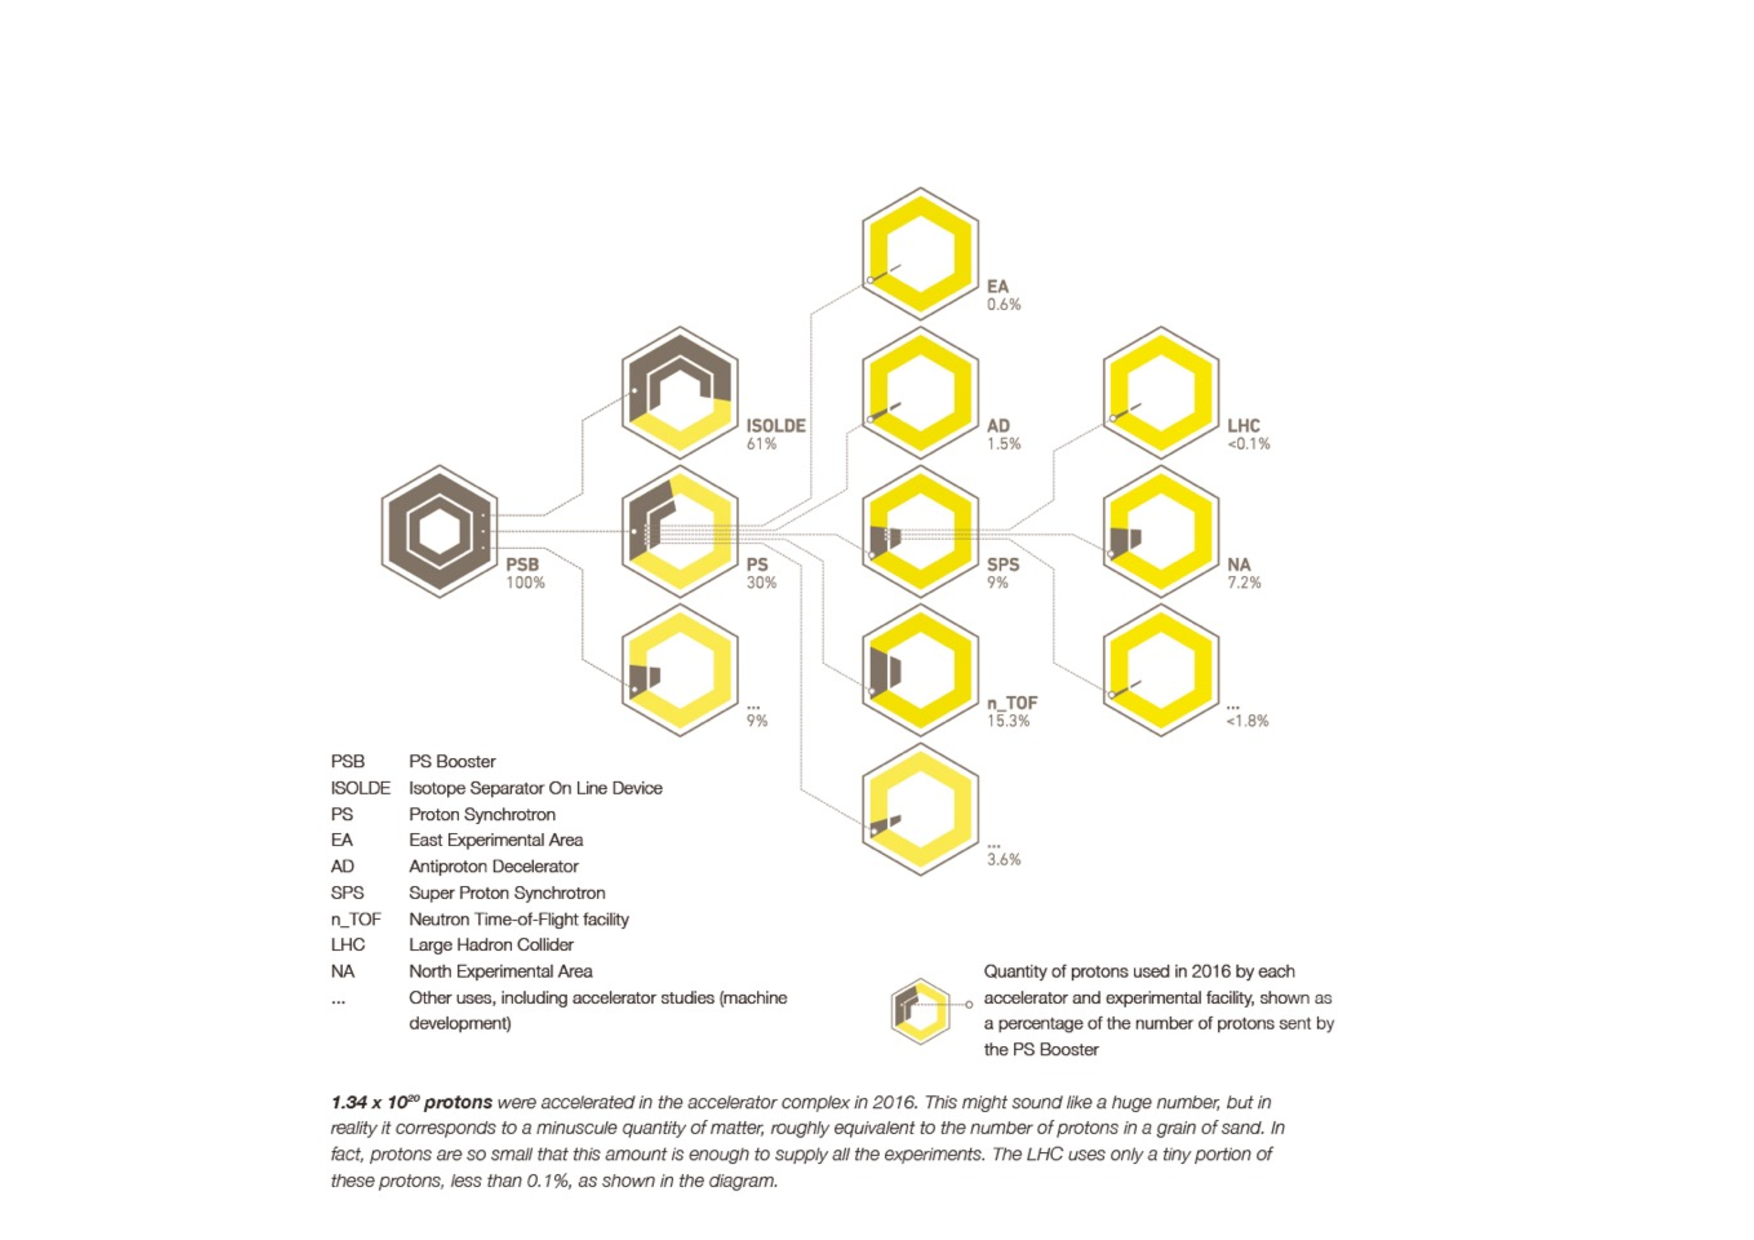
\includegraphics[width=0.8\textwidth]{figures/LHC/distribution_of_protons_en.pdf}
	\caption{Other experiments at the LHC accelerating chain~\cite{Pralavorio2017}}
	\label{fig:OtherExpAtAccStructure}
\end{figure}

The stages for proton acceleration are:
\begin{itemize}
    \item {\textit {\textbf {Grab proton source}}}: The Duoplasmatron~\cite{LHC-tdr-vol3} strips electron from the hydrogen gas and creates a plasma of protons, electrons and molecular ions. This plasma expands towards the extraction electrodes and a proton beam is formed. This feeds protons to the Linear accelerator-2 (LINAC2).
    \item {\textit {\textbf {LINAC2}}}: It is the starting point of proton's journey in the LHC accelerator complex. Here, proton beams are accelerated to an energy of 50 $MeV$ using the radio-frequency (RF) cavities\footnote{An RF cavity is a metallic cavity that accelerates the charged particles using the electromagnetic field.}. LINAC2 further feeds to the Proton Synchrotron Booster (PSB).
    \item {\textit {\textbf {PSB}}}: The 50 $MeV$ proton beams from LINAC2 are injected into the PSB. The PSB accelerates them to 1.4 $GeV$ for injection into the Proton Synchrotron (PS).
    \item {\textit {\textbf {PS}}}: It is one of the key components in the LHC accelerator complex. It increases the energy of protons up to 25 $GeV$ and feeds them to the Super Proton Synchrotron (SPS).
    \item {\textit {\textbf {SPS}}}: It has a circumference of 7 $km$ where protons are accelerated to an energy of 450 $GeV$. Protons are further injected into the LHC ring via two transmission lines.
    % Then via two transmission lines protons are further injected into the LHC ring.
    \item {\textit {\textbf {LHC}}}: It accepts the two proton beams from SPS which are injected into opposite directions in two parallel pipes. In LHC, proton beams can be accelerated up-to 7 $TeV$.
\end{itemize}
The CERN accelerator complex is shown in Figure~\ref{fig:CERN-accelerator-complex}.  
\begin{figure}[!htbp]
	\centering
	\includegraphics[width=1.15\textwidth,height=19cm]{figures/LHC/CERN_Accelerator_Complex-v2016.pdf}
	\caption{The LHC accelerator chain along with all its other experiments which use proton beam from different parts of the accelerator, either from PSB, PS or SPS~\cite{Fig-CERN-accelerator-complex}}
	\label{fig:CERN-accelerator-complex}
\end{figure}
% subsection accelerating_structure (end)
%%%%%%%%%%%%%%%%%%%%%%%%%%%%%%%%%%%%%%%%%%%%%%%%%%%%%%%%%%%%%%%%%%
%%%%%%%%%%%%%%%%%%%%%%%%%%%%%%%%%%%%%%%%%%%%%%%%%%%%%%%%%%%%%%%%%%
\subsection{Magnet System}
Since the LHC is a circular collider; the magnet system is one of its core parts as it provides a circular trajectory to the particles in the LHC beam pipes.
In order to be economical, LHC has been made in eight arcs and eight straight sections instead of a perfect circle.
To bend the beam dipole magnets are used. There are total of 1232 dipole magnets are used in LHC, having length 15 meter and weigh $\sim$ 35 tonnes, each~\cite{LHC:magnets_rossi}. A systematic diagram of LHC main dipole magnets along with its cold mass and vacuum chamber is shown in Fig.~\ref{fig:LHC_dipole}. Apart from bending the beam, it is also necessary to focus the proton beams.
\begin{figure}[!htbp]
	\centering
	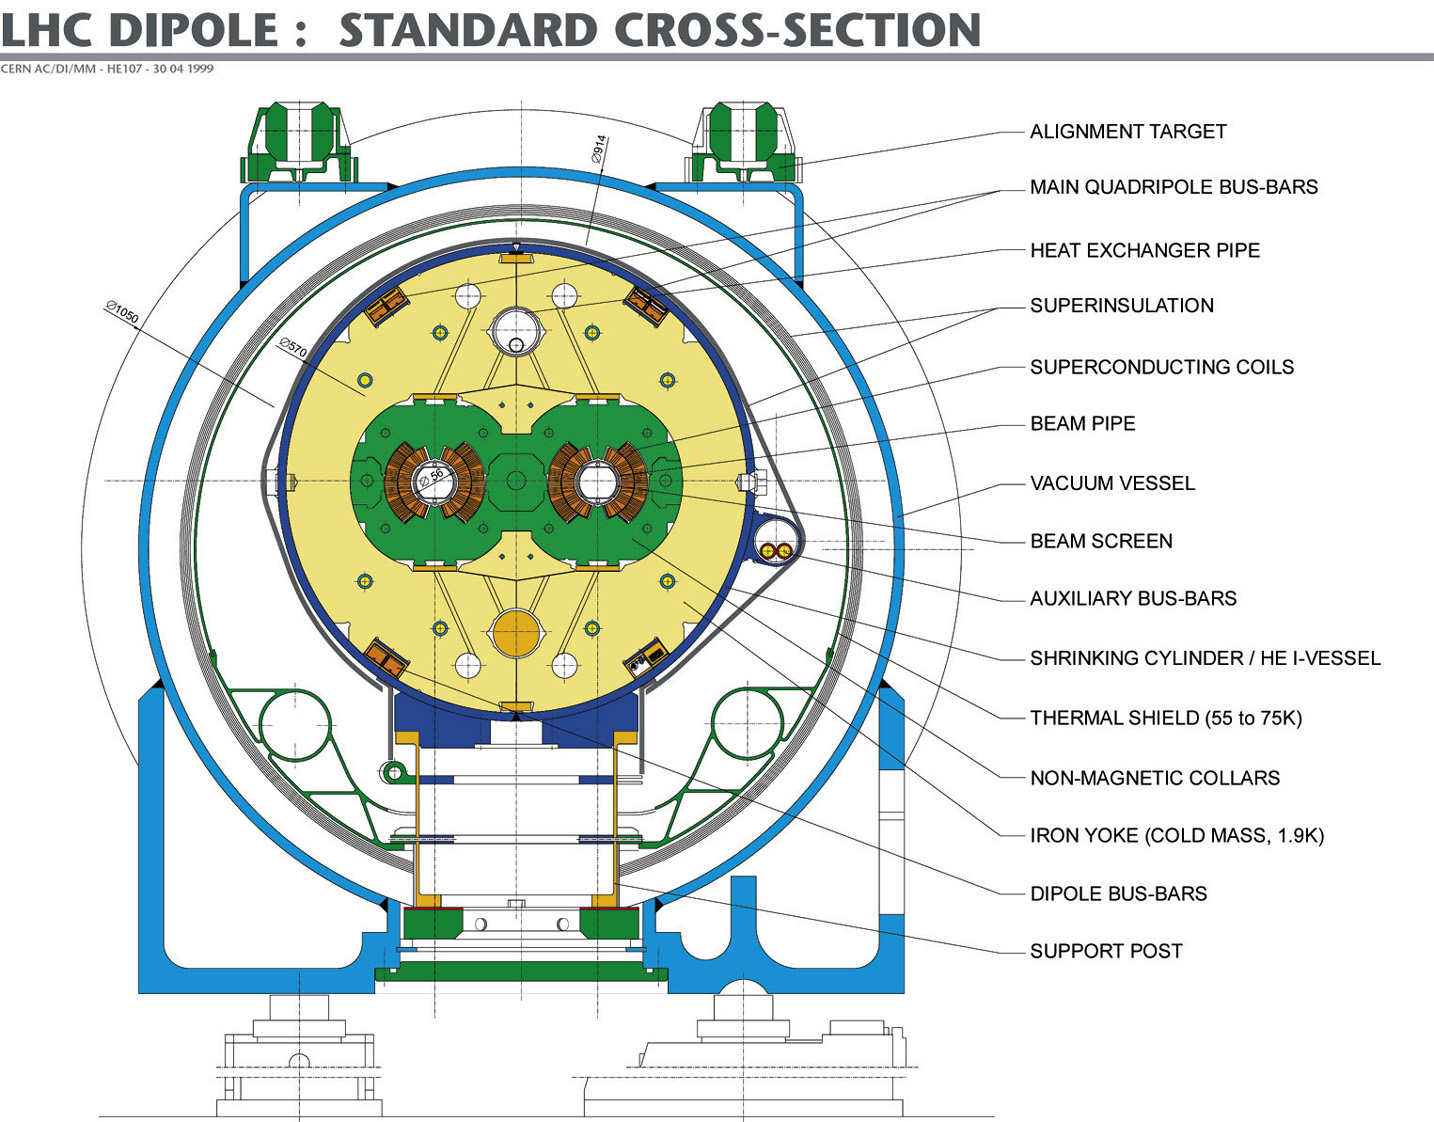
\includegraphics[width=0.95\textwidth]{figures/LHC/9906025_01.jpg}
	\caption{Diagram showing the cross-section of an LHC dipole magnet with cold mass and vacuum chamber~\cite{fig:40524}.}
	\label{fig:LHC_dipole}
\end{figure}
This is accomplished using a pair of quadrupole magnets, where the first magnet focuses the width while the second magnet focuses the beam height as shown in Figure~\ref{fig:QuadrupoleMagnet}.
A total of 858 quadrupole magnets are installed in LHC to keep the beams focused. 
\begin{figure}[!htbp]
	\centering
	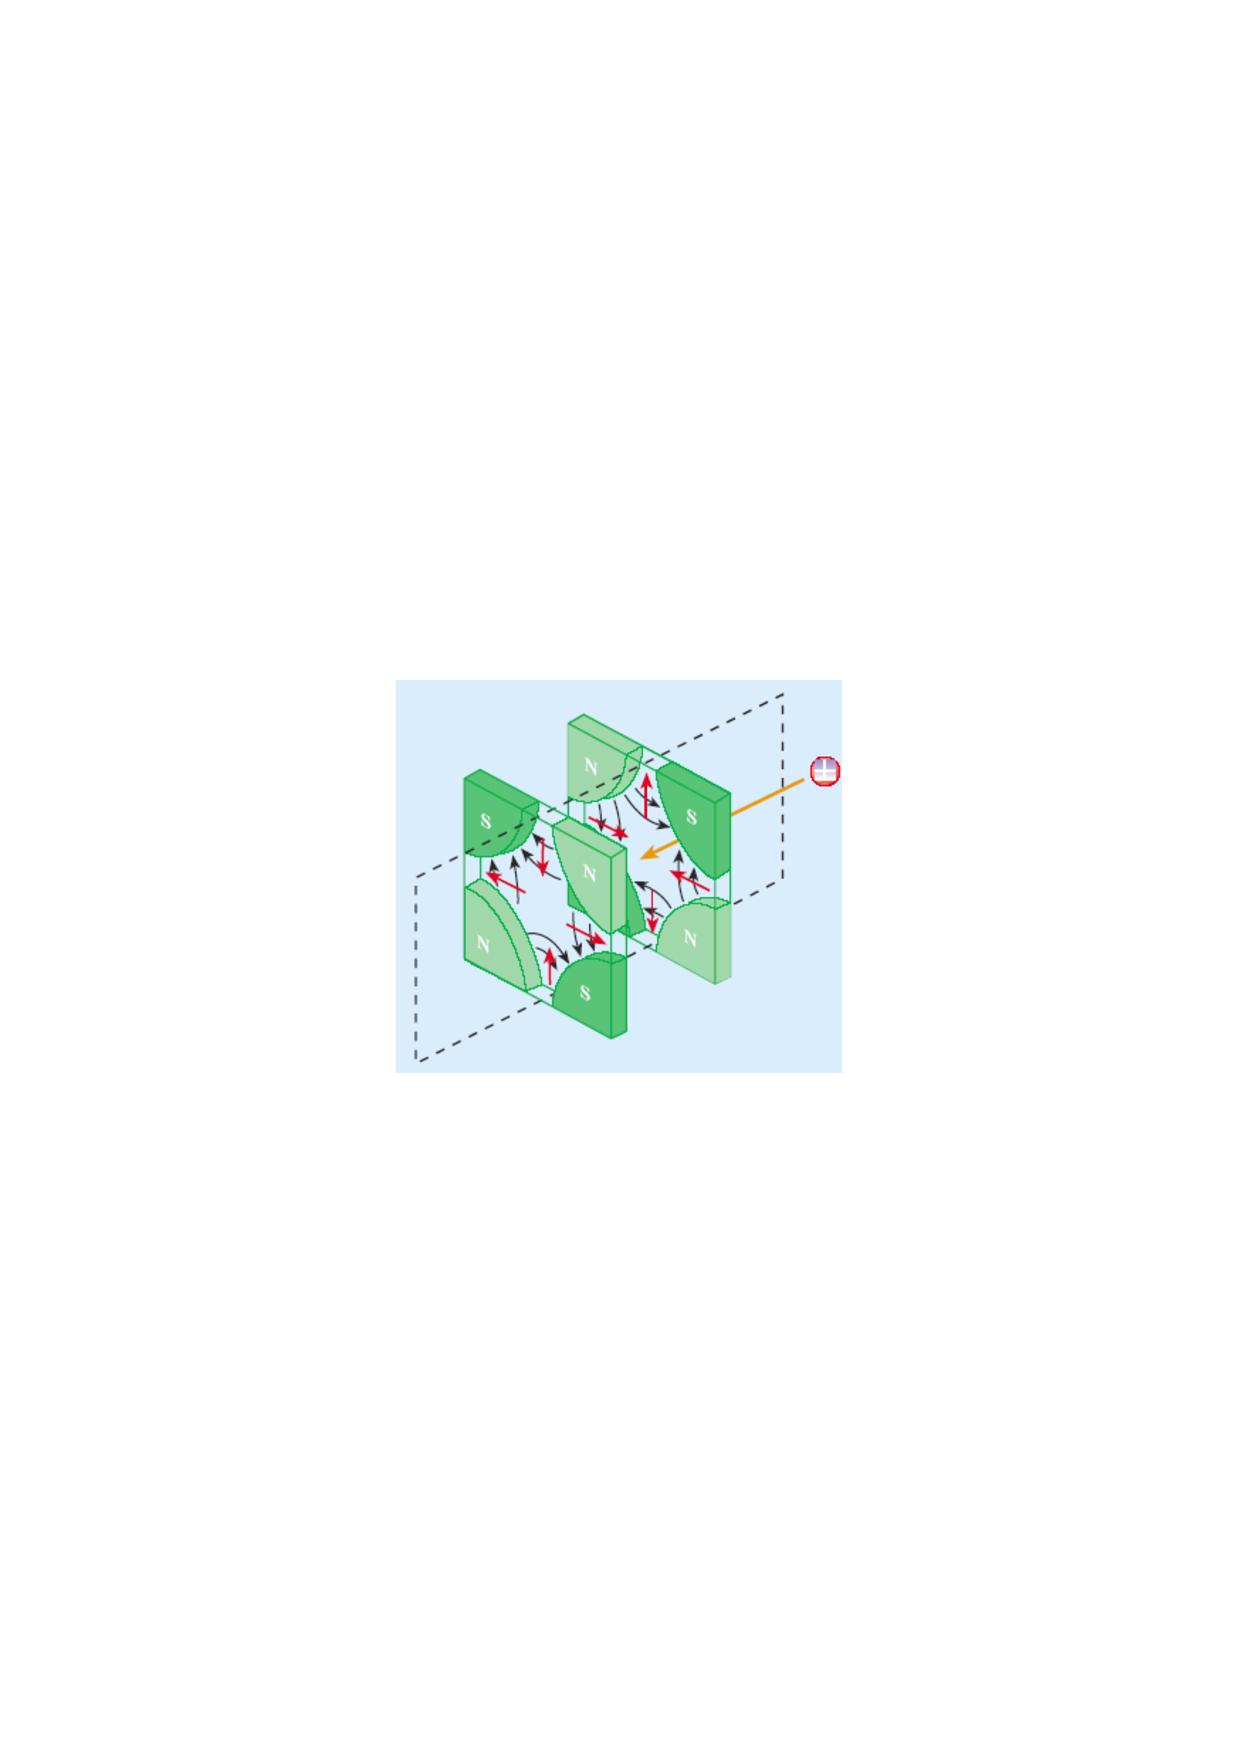
\includegraphics[width=0.50\textwidth]{figures/LHC/quadrupole_magnet_pair.pdf}
	\caption{Pair of quadrupole magnets~\cite{Vidal}.}
	\label{fig:QuadrupoleMagnet}
\end{figure}

Sextuple magnets are also used for proper focusing as every proton in the beam is not exactly with the same energy and on the same path. 
Several other magnetic multi-poles are used to keep the beam focused  in case the beam suffers from gravitational interactions over protons, electromagnetic interactions among bunches or electron clouds from pipe wall, and so on.
The details of the different types of magnets used in LHC are listed here \cite{WebLink:LHC_magnets}.
Besides, there are eight sets of ``\textit{inner triplets}" used at the four interaction points (IPs) to focus the beams during the collisions to increase the luminosity. The size of the bunch goes from 0.2 mm to 17 $\mu m$ and 71 $\mu m$ at the interaction point of ATLAS (A Toroidal LHC Apparatus) \& CMS (Compact Muon Solenoid) and ALICE (A Large Ion Collider Experiment) \& LHCb (Large Hadron Collider beauty), respectively. A list of important parameters of the LHC is given in Table~\ref{table:LHC-parameters}.

\begin{table}
% \vspace{-5.2em}
\centering
{\small
\begin{tabular}[!htbp]{l c}
\hline
{\textbf{Parameters}} & {\textbf{Value}} \\
\hline
Circumference of LHC ring   &   26658.883 m \\
\hline
Maximum dipole magnetic field   & 8.33 T \\
Dipole operating temperature    & 1.9 K \\
\hline
Maximum stored energy per beam (nominal) &   362 MJ \\
Maximum stored energy per beam  (2012) &   143 MJ \\
Maximum stored energy per beam  (2016) &   266 MJ \\
\hline
Beam energy at Injection    & 450 GeV \\
Beam energy at collision (nominal) &    7 TeV \\
Beam energy at collision (2012)     &   4 TeV \\
Beam energy at collision (2016)     &   6.5 TeV \\
\hline
Maximum instantaneous luminosity (nominal)  &   $10^{34}$ cm$^-2$ s$^{-1}$ \\
Maximum instantaneous luminosity (2012)     &   $7.7 \times 10^{33}$ cm$^-2$ s$^{-1}$ \\
Maximum instantaneous luminosity (2016)     &   $1.4 \times 10^{34}$ cm$^-2$ s$^{-1}$ \\
\hline
Number of bunches per proton beam (nominal) &   2808 \\
Number of bunches per proton beam (2012)    &   1380 \\
Number of bunches per proton beam (2016)    &   2076 \\
Maximum number of protons per bunch         &   $1.6 \times 10^{11}$ \\
\hline
Protons/bunch (average at start of collision) (nominal)   &   $1.15 \times 10^{11}$ \\
Protons/bunch (average at start of collision) (2012)  &   $1.5 \times 10^{11}$ \\
Protons/bunch (average at start of collision) (2016)  &   $1.1 \times 10^{11}$ \\
\hline
Bunch collision frequency (nominal)         &   40 MHz  \\
Bunch collision frequency (2012)            &   20 MHz  \\
Bunch collision frequency (2016)            &   40 MHz  \\
\hline
Bunch length (at injection)   &   1.7 ns \\
Bunch length (at collision)   &   1.05 ns \\
Energy spread (at injection)   &   1.9$\times 10^{-3}$ \\
Energy spread (at collision)   &   0.45$\times 10^{-3}$  \\
\hline
Half crossing angle  (nominal)   & 143 $\mu rad$ \\
Half crossing angle  (2012)   & 146 $\mu rad$ \\
Half crossing angle  (2016)   & 185 $\mu rad$ \\
\hline
$\beta *$  (nominal) &   0.55 m\\
$\beta *$   (2012)&   0.6 m\\
$\beta *$   (2016)&   0.4 m\\
\hline
RMS beam size at IP1 \& IP5 &   17 $\mu m$ \\
RMS beam size at IP2 \& IP8 &   71 $\mu m$ \\
\hline
$\epsilon_n$(transverse emittance, RMS, normalized) (at injection) &   3.5 $\mu$m\\
$\epsilon_n$(transverse emittance, RMS, normalized) (at collision point) &   3.75 $\mu$m\\
\hline
total longitudinal emittance (at injection) & 1.0 eVs \\
total longitudinal emittance (at collision) & 2.5 eVs \\
\hline
Average mean pile-up (nominal) &   25 \\
Average mean pile-up (2012) &    21 \\
Average mean pile-up (2016) &    27 \\
\hline
Energy loss per turn at 14 TeV              &   7 keV   \\
Energy loss per turn for electrons at 104.6 GeV          &  40,000 keV     \\
\hline
% synchtron radiation for electrons: Reference: Particle Physics Experiments at high energy colliders by John Hauptman
\end{tabular}
\caption{LHC technical parameters for proton-proton collisions: nominal, 2012 and 2016 values.\cite{Bruce2016, Schoerner-Sadenius2015, LHC-parameters-2016, LHC-tdr-vol1, cms-lumi-public-results}.}
\label{table:LHC-parameters}
}
\end{table}

%%%%%%%%%%%%%%%%%%%%%%%%%%%%%%%%%%%%%%%%%%%%%%%%%%%%%%%%%%%%%%%%%%
%%%%%%%%%%%%%%%%%%%%%%%%%%%%%%%%%%%%%%%%%%%%%%%%%%%%%%%%%%%%%%%%%%
\section{Key requirements of a particle accelerator} % (fold)
\label{sub:few_key_requirements}

The HEP collider is characterised on the basis of two parameters - the centre of mass energy and the luminosity. 
The production rate of heavier particles like Higgs increases with the centre of mass energy. 
Luminosity ({$\Lagr$}) measures the ability of a collider to produce the required number of interactions. It is the proportionality factor between the number of events per second $dR/dt$ and the cross-section $\sigma_p$~\cite{Muratori2006}.
\begin{equation}
	\frac{dR}{dt} = \Lagr ~~.~~ \sigma_p~,
\end{equation}
The unit of luminosity is $cm^{-2}s^{-1}$.

\subsubsection{Luminosity calculation} % (fold)
\label{ssub:luminosity_calculation}
Luminosity is defined as:
\begin{equation}
    \Lagr = \frac{k_bN_1N_2f_{rev}\gamma}{A_{eff}}~,
\end{equation}
Where, $k_b$ is the number of bunches per beam, $N_1$ and $N_2$ are the number of protons in the two bunches, $f_{rev}$ the revolution frequency of proton beams, $\gamma$ is the geometric factor and $A_{eff}$ is the effective transverse area of the beam. The different parameters of the beam as showing in the Fig.~\ref{fig:lumi}.
\begin{figure}[!htbp]
	\centering
	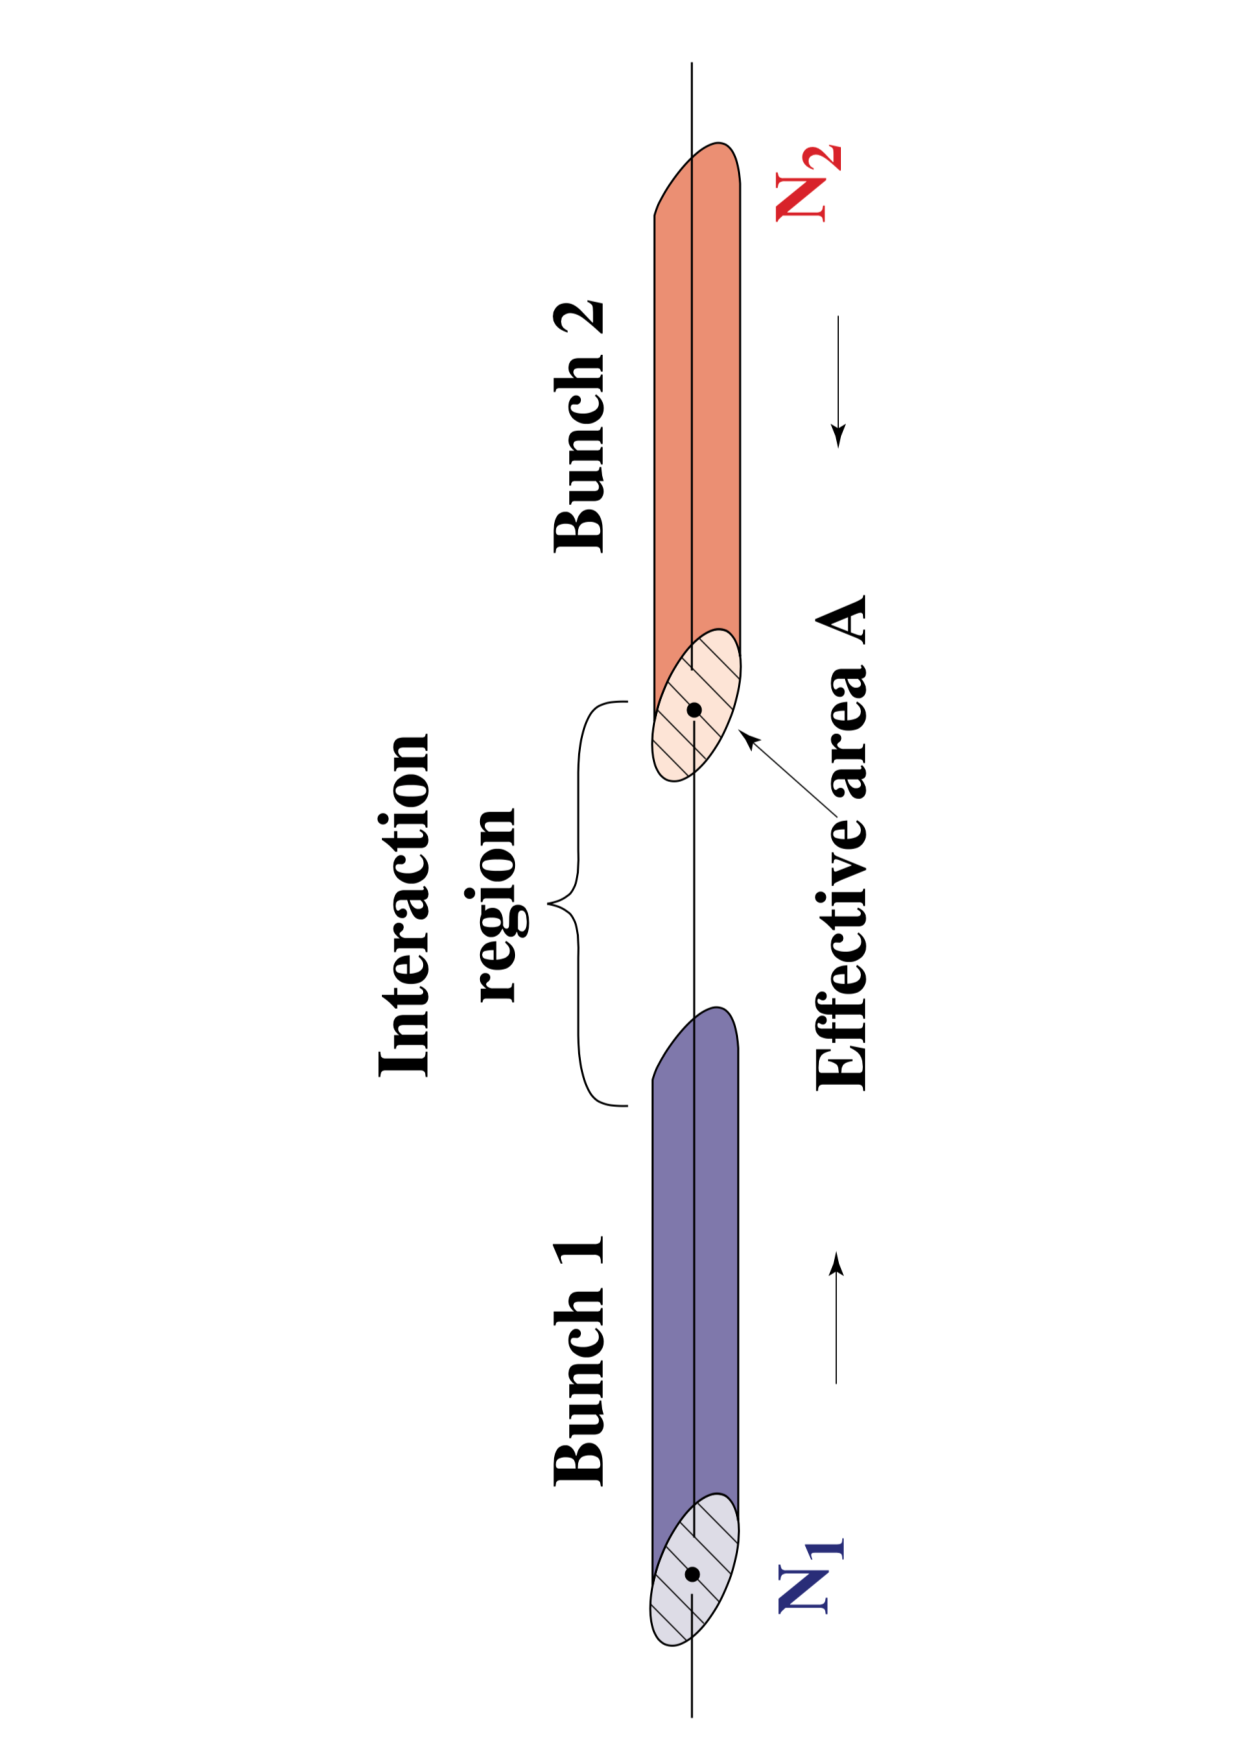
\includegraphics[width=0.95\textwidth]{figures/LHC/Luminosity_calculation.pdf}
	\caption{Layout describing the bunch parameters and interaction area.}
	\label{fig:lumi}
\end{figure}
The geometric factor $\gamma$ is given by
\begin{equation}
	\gamma = \frac{1}{\sqrt{1+(\frac{\sigma_s}{\sigma_{xing}}\frac{\alpha}{2})^2}}
\end{equation}
where $\sigma_s$ is the r.m.s. bunch length, $\sigma_{xing}$ is the transverse beam size in the crossing plane, and $\alpha/2$ is the half crossing angle~\cite{Hostettler2017}.
% The luminosity is proportional to the number of events per second so it should be maximised. Luminosity is the 
% \hspace{2 cm}$\epsilon_n$ is the normalised RMS transverse beam emittance (same in both )\\
% \hspace{2 cm}$\beta^*$ is the beta-function at the interaction point\\
For a Gaussian beam with spread $\sigma_x$ and $\sigma_y$ in x and y direction respectively, the effective area will be $4\pi \sigma_x \sigma_y$, so that
\begin{equation}\label{eq:luminosity}
    \Lagr = \frac{k_bN_1N_2f_{rev}\gamma}{4 \pi \sigma_x \sigma_y}~,
\end{equation}
The beam size, $\sigma_x~.~\sigma_y$, can be expressed in terms of transverse beam emittance\footnote{The transverse emittance is a beam quality concept reflecting the process of bunch preparation (the injector chain), extending all the way back to the source for hadrons. A low emittance particle beam is a beam where the particles are confined to a small distance and have nearly the same momentum. In a colliding beam accelerator, keeping the emittance small means that the likelihood of particle interactions will be greater resulting in higher luminosity. The emittance changes as a function of the beam momentum; increasing the energy of the beam reduces the emittance.} ($\epsilon_n$) and the amplitude function\footnote{The amplitude function, $\beta^*$ , is determined by the accelerator magnet configuration (basically, the quadrupole magnet arrangement) and powering. } ($\beta^*$, also known as beta-function). The amplitude function can be expressed in terms of cross-sectional size of the bunch ($\sigma_x~.~\sigma_y$) and  the transverse emittance ($\epsilon_n$). The amplitude function $\beta$  becomes 
\begin{equation}\label{eq:beta_function}
	\beta^* = \frac{\pi.\sigma_x.\sigma_y}{\epsilon_n}~,
\end{equation}. 
If the amplitude function is small, the beam will be narrower and squeezed. If it is high, the beam will be wide and straight. It has unit of length. Thus, we can express luminosity in terms of transverse emittance and the amplitude function as
\begin{equation}\label{eq:luminosity2}
    \Lagr = \frac{k_bN_1N_2f_{rev}\gamma}{4 \pi \epsilon_n \beta^*}~,
\end{equation}
Based on the definition of luminosity, we can maximise it by following ways:
\begin{itemize}
    \item By decreasing beam emittance, $\epsilon_n$.
    \item By improving the cryogenic system as the factor $k_b~.~N_1~.~N_2$ is limited by thermal energy produced by synchrotron radiation.
    \item By decreasing beam-beam effect~\cite{Herr2014,Papotti2014}, since it scales with $N_b/ \epsilon_n$ which causes the spread in betatron tunes~\cite{Dubouchet2013}.
    \item Also, the space charge~\cite{Oeftiger2016} scales with $N_b/ \epsilon_n$.
\end{itemize}
% subsubsection luminosity_calculation (end)

\subsubsection{Integrated luminosity} % (fold)
\label{ssub:integrated_luminosity}
The maximum luminosity or the instantaneous luminosity is an important quantity but the final figure of merit is the \textbf{integrated luminosity} as it directly gives us the total number of observed events over a period of time:
\begin{equation}
	\Lagr_{int}~.~\sigma_p = number~of~events~of~interest~,
\end{equation}
where, $L_{int}$ is defined as the integral of the delivered luminosity over time. It is the measurement of the collected data size.
\begin{equation}
	\Lagr_{int} = \int_0^T L(t')dt'~,
\end{equation}
Its unit is $barn^{-1}$. Figure~\ref{fig:lumi-proj-2016-final-v2} shows the integrated luminosity of 2016 as compared to the previous years.
\begin{figure}[!htbp]
	\centering
	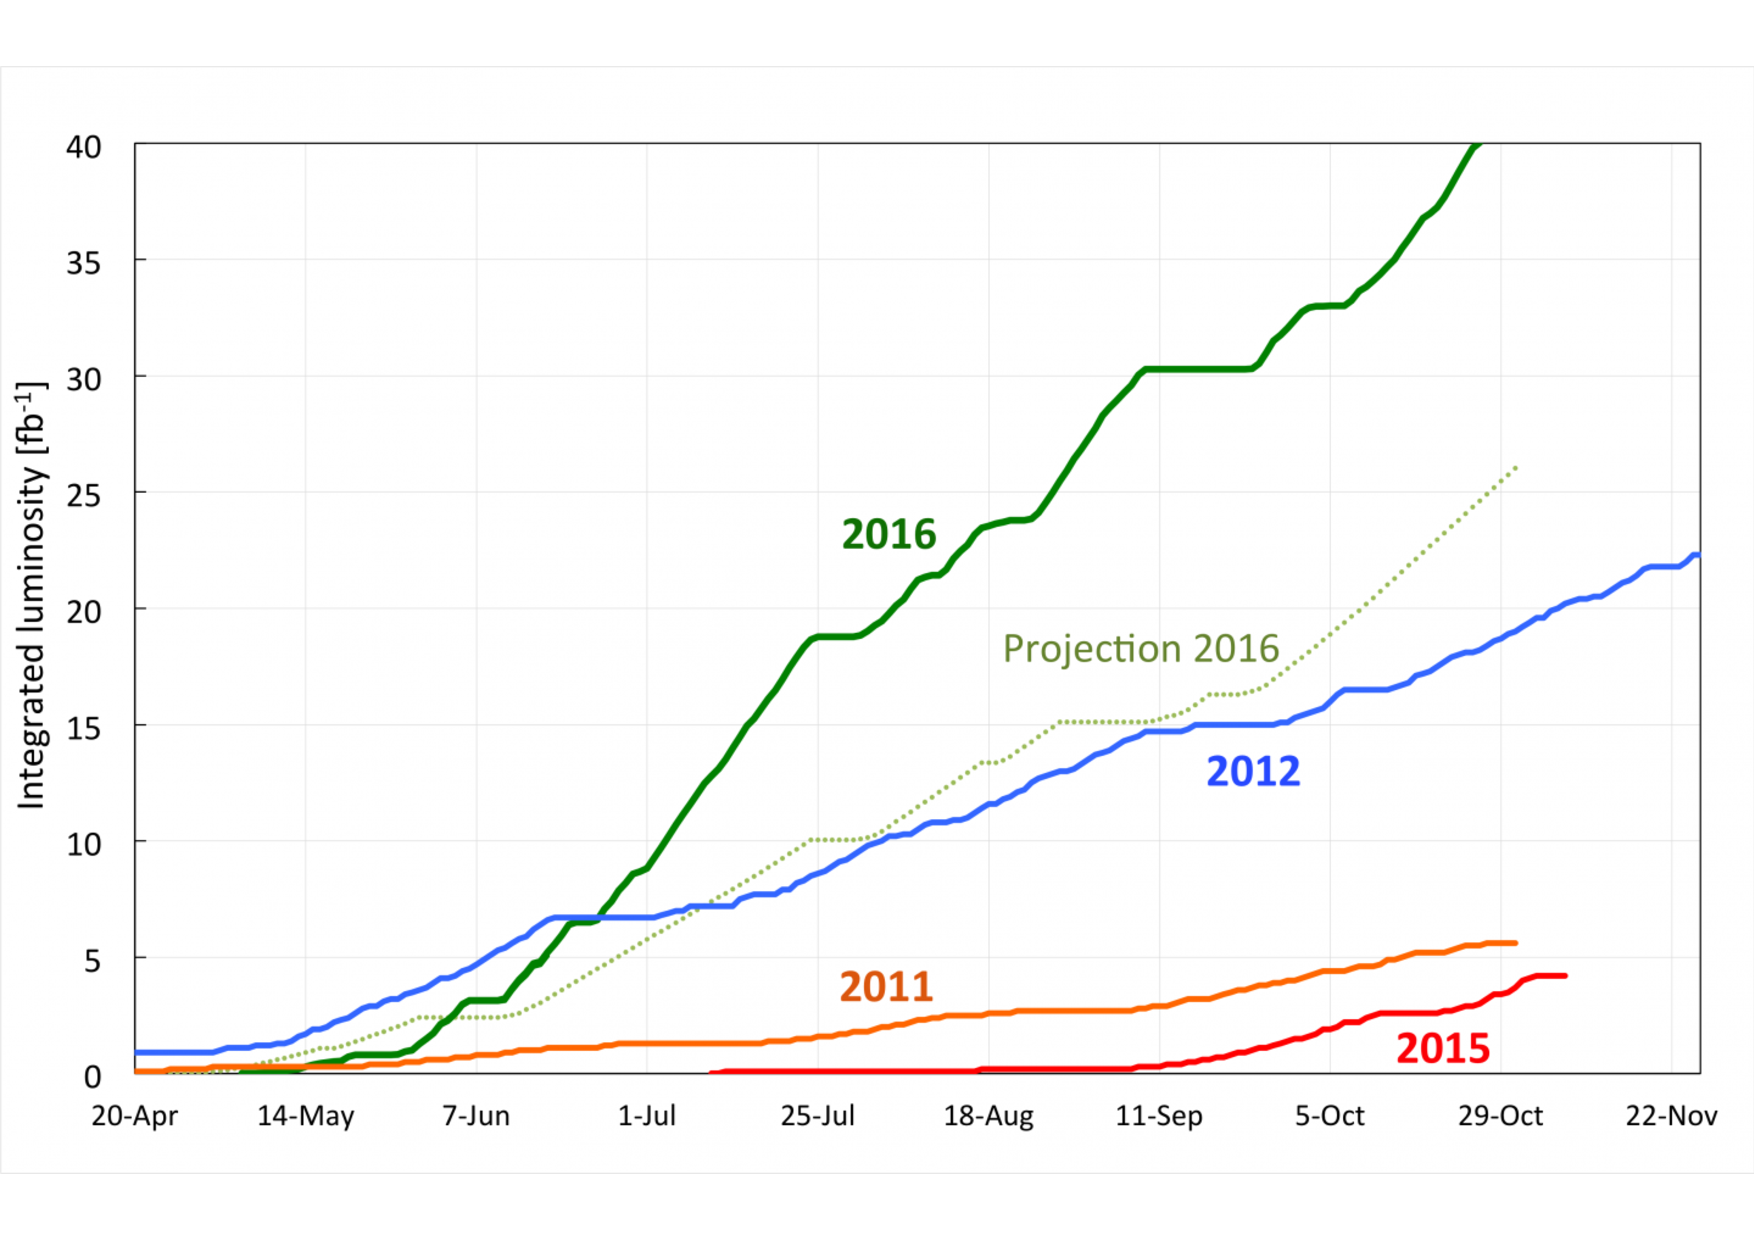
\includegraphics[width=0.75\textwidth]{figures/lumi-proj-2016-final-v2.pdf}
	\caption{The integrated luminosity of the LHC with proton-proton collisions in 2016 compared to previous years~\cite{Pralavorio2016}. The recorded luminosity in 2016 far surpassed the expected luminosity and it almost doubled the luminosity recorded in 2012.\todo[inline]{explain each line}}
	\label{fig:lumi-proj-2016-final-v2}
\end{figure}
% subsubsection integrated_luminosity (end)
\todo[inline]{Add luminosity measurement section}
% subsection few_key_requirements (end)
% section the_large_hadron_collider (end)

%%%%%%%%%%%%%%%%%%%%%%%%%%%%%%%%%%%%%%%%%%%%%%%%%%%%%%%%%%%%%%%%%%
\section{Experiments at the LHC} % (fold)
\label{sec:experiments_at_the_lhc}

At the LHC there are four IPs where the two proton beams are made to collide. At each IP, one detector is placed. These are - ATLAS, CMS, ALICE, and LHCb as shown in Figure~\ref{fig:LHCgeometry}.
\begin{figure}[!htbp]
	\centering
	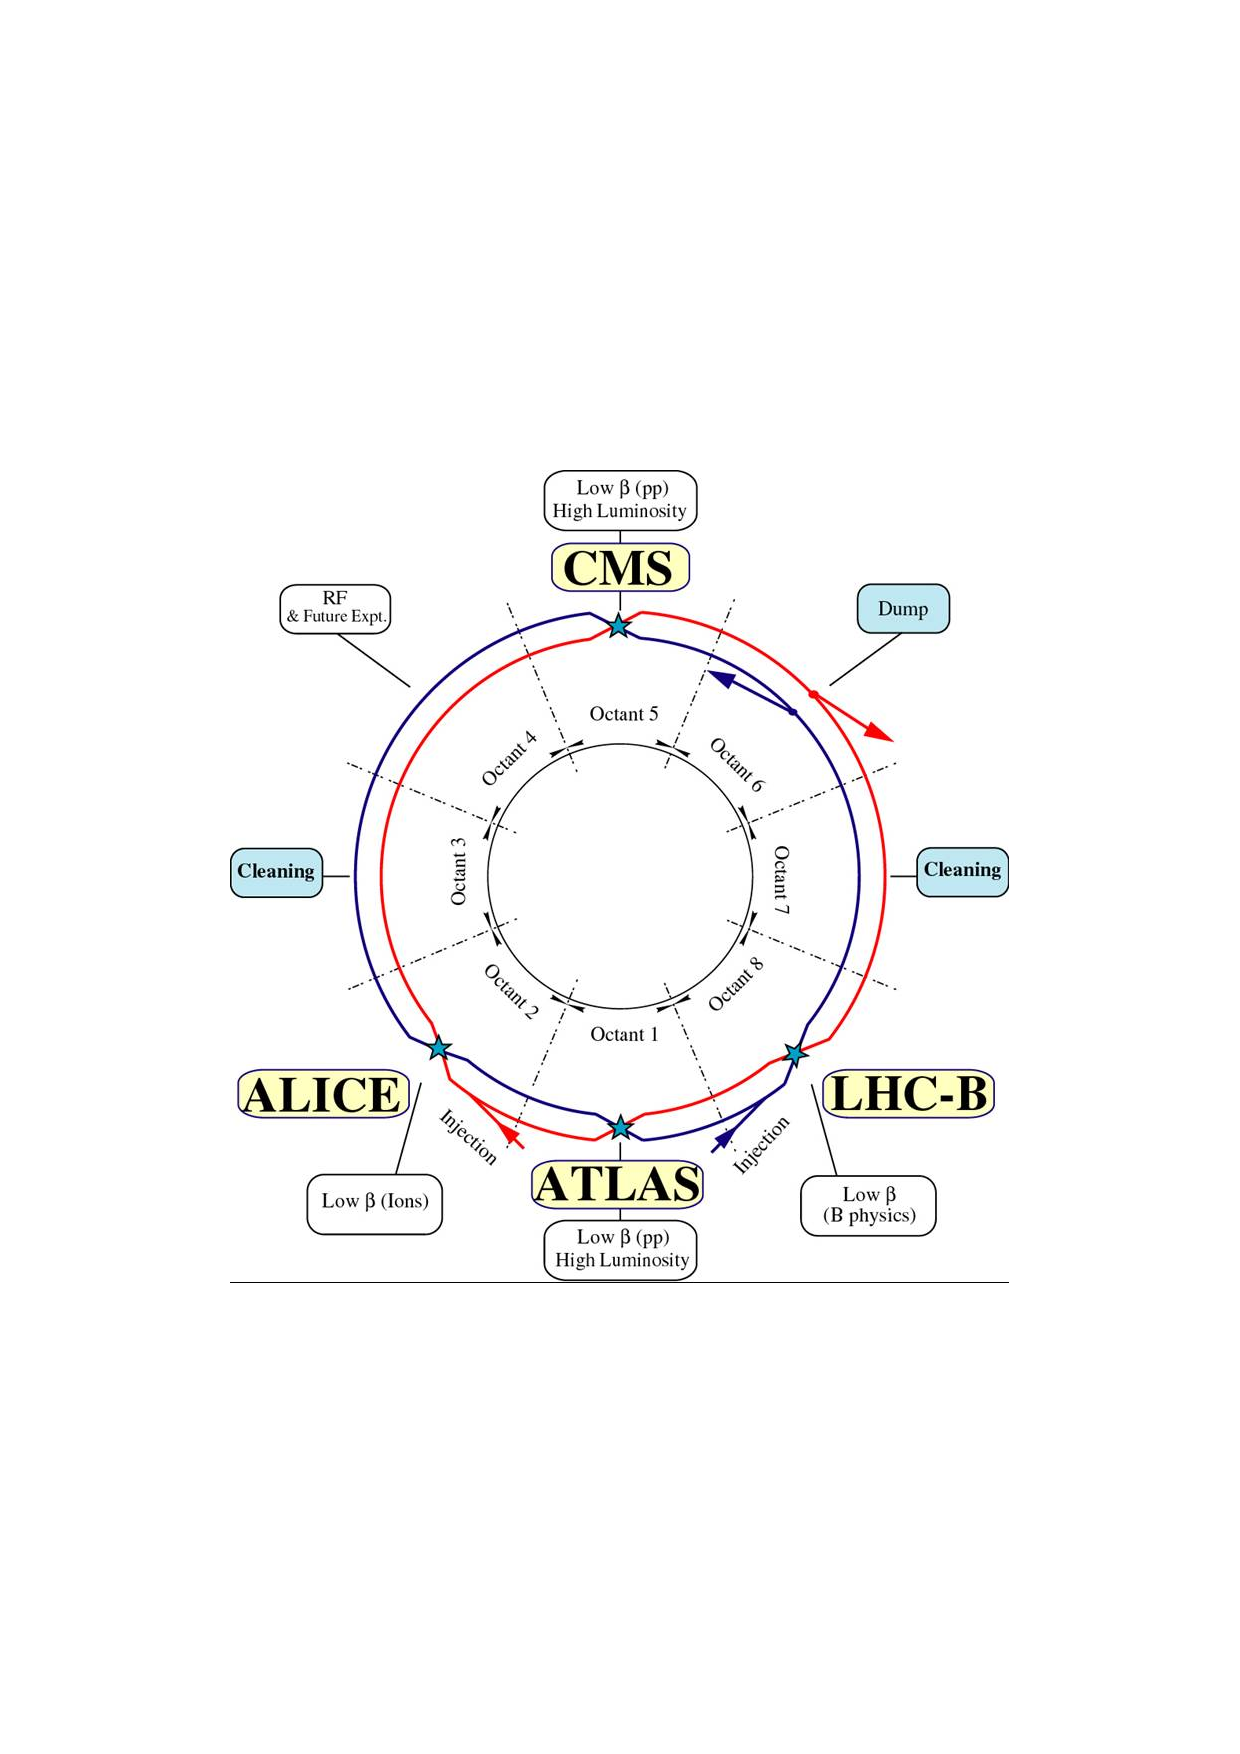
\includegraphics[width=0.81\textwidth,height=9.5cm]{figures/LHC/lhc-schematic.pdf}
	\caption{LHC geometry with arcs and straight sections~\cite{CERN}.}
	\label{fig:LHCgeometry}
\end{figure}
In addition to these, there are two more small detectors LHCf and TOTEM installed close to the IP of the two main detectors ATLAS and CMS respectively.\\
{\textbf{ATLAS}} (A Toroidal LHC Apparatus) and {\textbf{CMS}} (Compact Muon Solenoid) are large general-purpose\footnote{Here, general purpose means this machines will be used for many different kind of physics searches.} detectors with similar design and physics goal. 
The main difference between the two is in their magnet systems which is motivated by the momentum resolution of muons. 
The momentum resolution for muons, $\Delta p_T/p_T$, is proportional to  $B^{-1}L^{-2}$, where B is magnetic field and L is the lever arm defined as the distance of momentum measurement from the IP of detector. 
So, to improve the momentum resolution there are three possible choices.

\begin{enumerate}
	\item To increase $B$ while maintaining a compact design, or
	\item To work with low $B$ with long $L$, and
	\item To increase both $L$ and $B$, but this increases the cost of the detector by several factors. Hence, it is not the preferred choice usually.
\end{enumerate}

CMS uses the first point, i.e., to increase the magnetic field with compact design\footnote{This is why there is word {\textbf{compact}} in the name of CMS.} while ATLAS uses the design with low magnetic field with long lever arm.

% ATLAS has an eight toroidal magnets combined with a smaller inner solenoid while CMS has a powerful solenoid magnet only.

{\textbf{ALICE}} (A Large Ion Collider Experiment) is a heavy-ion detector. It is specially designed for the study of strongly interacting matter at high densities in quark-gluon plasma phase.

{\textbf{LHCb}} (Large Hadron Collider beauty) is made asymmetrically with respect to the IP of the detector. It is designed specially to investigate the matter-antimatter asymmetry through the study of b-quarks.

{\textbf{LHCf}} (Large Hadron Collider forward) and {\textbf{TOTEM}} (TOTal cross-section, Elastic scattering and diffraction dissociation Measurement at the LHC) are there for the study of forward physics\todo[inline]{define forward physics}.
% section experiments_at_the_lhc (end)

% %%%%%%%%%%%%%%%%%%%%%%%%%%%%%%%%%%%%%%%%%%%%%%%%%%%%%%%%%%%%%%%%%%
\section{CMS Detector} % (fold)
\label{sec:cms_experiment}
The design and components of any HEP detector depend upon its physics goals and operational parameters of the particle accelerator where it is installed. In case of the CMS detector, following challenges are imposed by the LHC accelerator:
\begin{enumerate}
	\item \textbf{ \textit{High luminosity}}: A high delivered luminosity implies that whenever two proton bunches cross each other there will be more than one p-p interactions also known as ``\textit{pile-up}''\footnote{Pile-up can be theoretically estimated as the product of inelastic p-p cross-section ($\sigma_{inel}$), instantaneous luminosity ($\Lagr$) and the mean time interval between two collisions, ($< t >$). \begin{equation}
		mean~pile-up = \sigma_{inel} \times \Lagr \times <t>~,
	\end{equation}}. Figure~\ref{fig:pile-up} shows the mean number of interactions for year 2016 and previous years. Given this, there will be more than $\mathcal{O}(1000)$ particles passing through detector during every p-p collision.\todo[inline]{update previous line} Thus, the detector should be highly granular which means an increased number of readout channels, synchronised with LHC clock.
	\item \textbf{\textit{Response time}}: At LHC, the two proton beams cross each other at every 25 ns. So, the response time of all the sub-detector systems should be less than 25 ns.
	\item \textbf{\textit{Radiation hardness}}: At every 25 ns, the detector is bombarded with more than 1000 particles so all the sub-detectors should be radiation hard including its electronics, cables, glue, screws, and so on.
\end{enumerate}
\begin{figure}[!htbp]
	\centering
	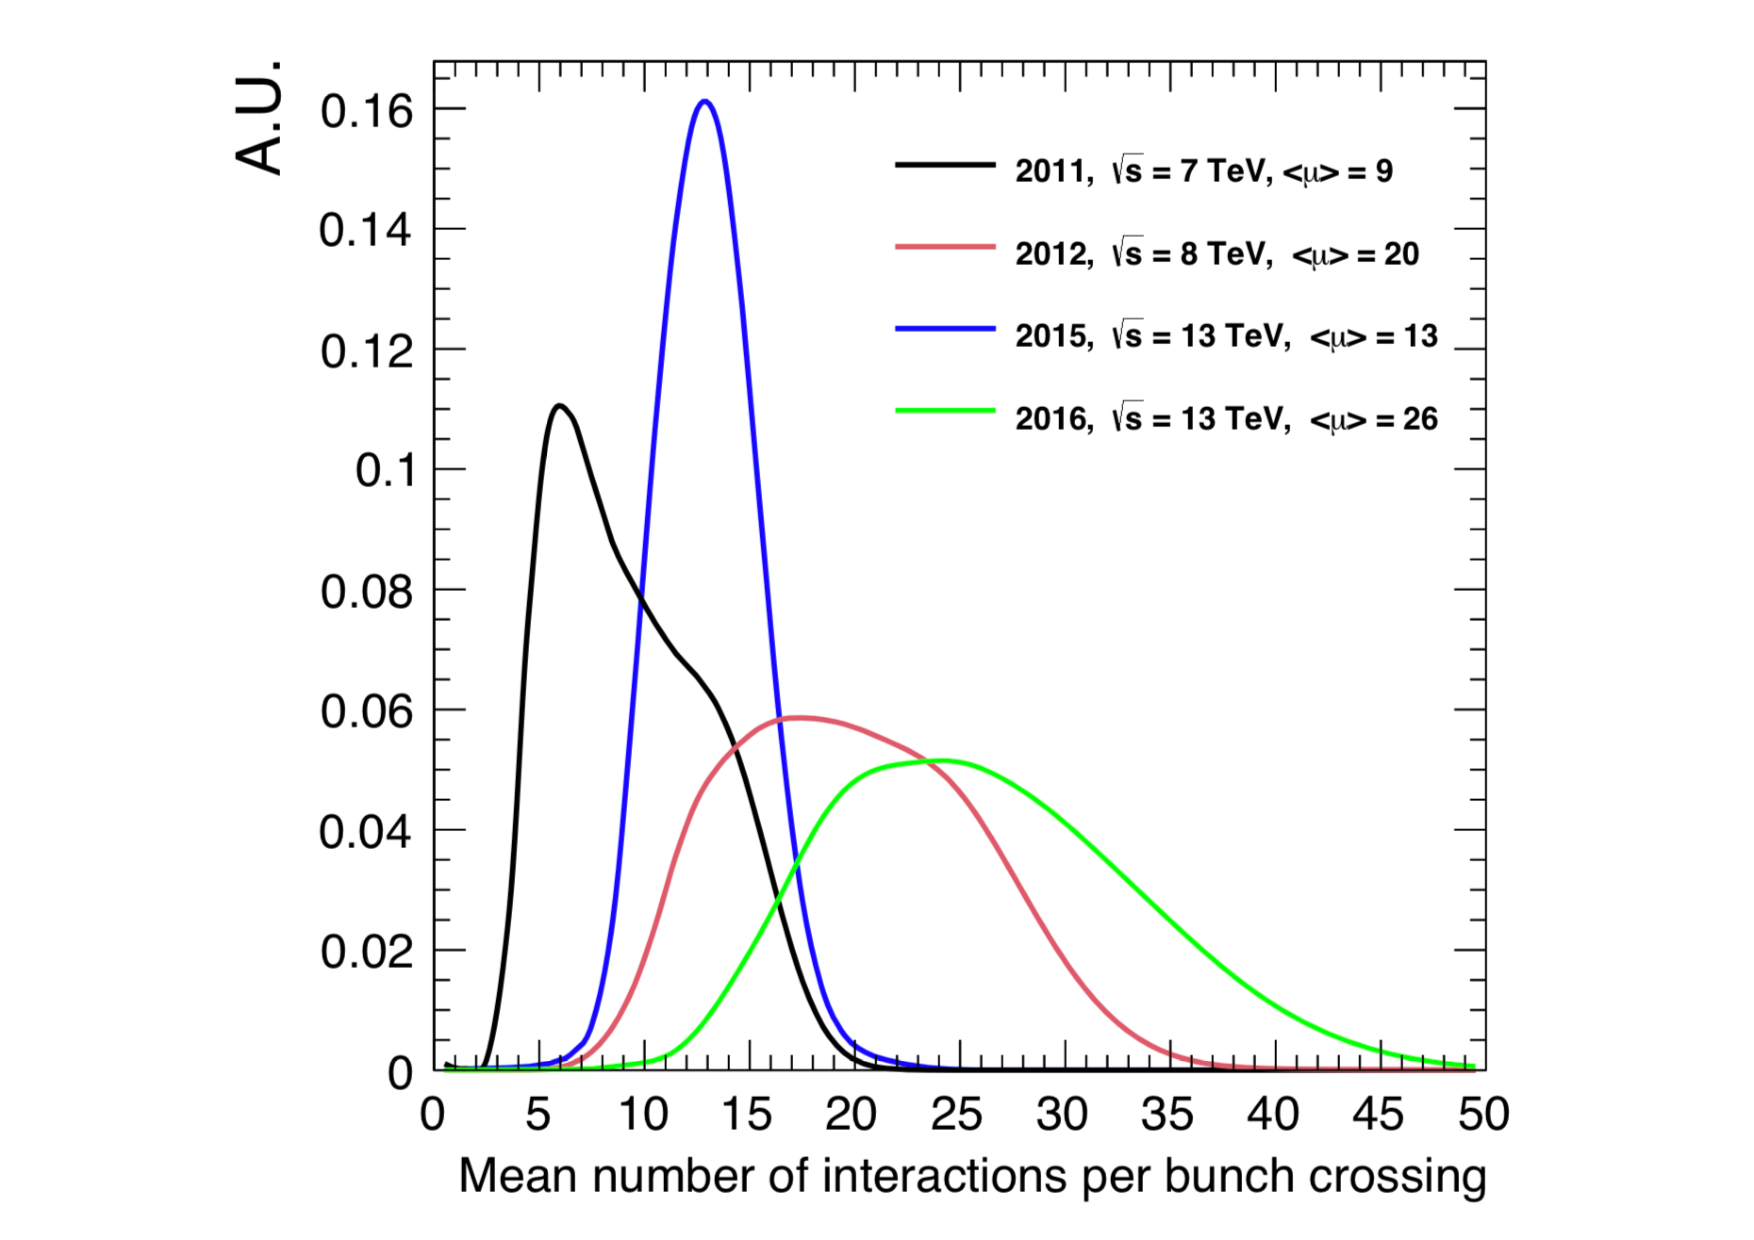
\includegraphics[width=0.60\textwidth]{figures/LHC/pileup.pdf}
	\caption{Mean number of interactions per bunch crossing in p-p collision~\cite{Apyan2017}.}
	\label{fig:pile-up}
\end{figure}
Restrictions imposed on detector from the physics goals of the LHC:
\begin{enumerate}
	\item Good muon identification and momentum resolution ($\approx$ 1\% at 100 GeV).
	\item Efficient triggering and tracking of b-jets and $\tau$'s.
	\item Highly efficient and granular electromagnetic calorimeter to detect and measure energies of electrons and photons.
	\item Good missing transverse energy resolution and di-jet mass resolution require a ``hermetic'' hadron calorimeter with full geometric coverage and fine lateral segmentation.
\end{enumerate}
% When the two beam of proton collides then thousands of particles are produced and out of them only 9 particles are of interest from detector construction point of view. They are photons ($\gamma$), electrons ($e$), muons ($\mu$), pions ($\pi^{\pm}$), kaon ($K^{\pm},~K_L,~K_S$), protons ($p$), and neutrons ($n$). Out of rest there are three neutrinos which interacts only weakly that do not interact in light mass HEP detectors and others are short lived particles. So, 
Based on the above conditions the CMS detector is designed in a cylindrical shape such that each sub-detector component is on top of the other, with the beam pipe at the centre. 
To have a full geometric coverage, it is designed with a barrel region and two endcap regions. The main part of the CMS detector is its superconducting magnet system, capable of producing a highly uniform magnetic field of 4T to accurately measure the high momentum particles. 
While the muon detector system is kept outside the magnet but sandwiched in its return yoke, the tracking system, the calorimeters Electromagnetic CALorimeter (ECAL) and Hadronic CALorimeter (HCAL) are placed inside the magnet.
The CMS detector design is shown in Figure~\ref{fig:CMS-detector}.
\begin{figure}[!htbp]
	\centering
	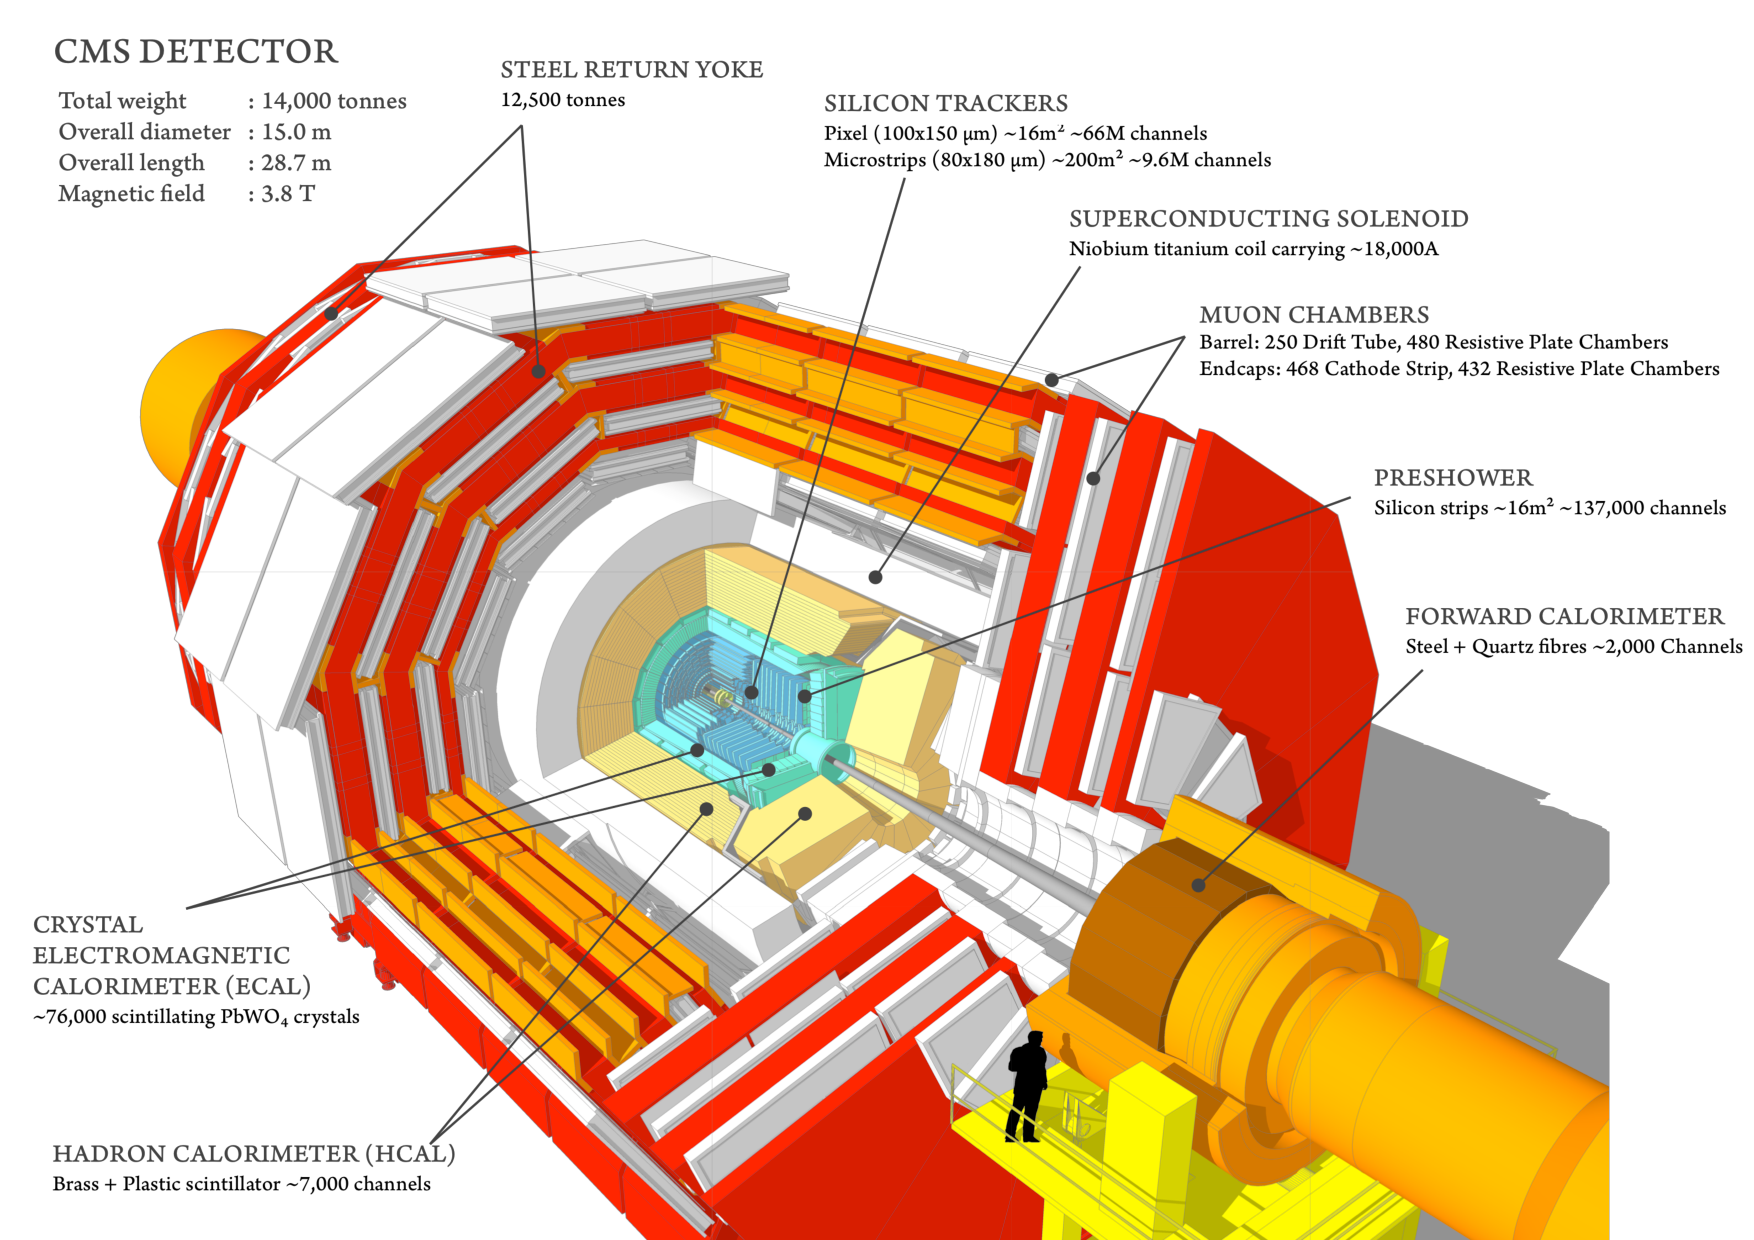
\includegraphics[width=1.1\textwidth]{figures/LHC/cms_120918_03.pdf}
	\caption{CMS detector drawing~\cite{Taylor2011}.}
	\label{fig:CMS-detector}
\end{figure}

The above mentioned shape of CMS was inspired by all the known particles that will reach to the CMS detector.
The known particle that will reach CMS detector are $e^{\pm}$, $\mu^{\pm}$, $\gamma$, $\pi^{\pm}$, K$^{\pm}$, p, n, $k_{L}$ and $k_{S}$.
These can be grouped in two categories based on electromagnetic and strong interactions.
All the strongly interacting particles will be detected by HCAL while all the electromagnetic interacting particles should be detected by ECAL.
But only electrons and photons are detected by ECAL not muons.
As it will not bremsstrahlung because it is too heavy than electrons (as bremsstrahlung is inversely proportional to $mass^4$).
Since muons can not interact via strong force it will pass through ECAL as well as HCAL.
Thus CMS is installed in a separate muon system outside ECAL and HCAL.

\subsection{Coordinate System} % (fold)
\label{sub:coordinate_system}
The right handed coordinate system is used in the CMS detector having origin at the nominal IP (Figure~\ref{fig:cms-coordinate-system}). The z-axis is considered along the beam direction in a way that x-axis and y-axis point radially to the centre of the LHC ring and in upward direction, respectively. The azimuthal angle, $\phi$, is measured in the x-y plane from x-axis and the polar angle, $\theta$, is measured from the z-axis. Instead of describing a particle at some polar angle, we prefer to use the variable pseudo-rapidity. It is defined as 
\begin{equation}
	\eta = -ln\bigg[tan\Big(\frac{\theta}{2}\Big)\bigg]~,
\end{equation}
In the hadron collider, the use of pseudo-rapidity was motivated from the invariance of its difference, $\Delta \eta$, with respect to the particle boost direction. Also, the particle density remains constant in the barrel region of the detector, measured in equal rapidity intervals.

\begin{figure}[!htbp]
	\centering
	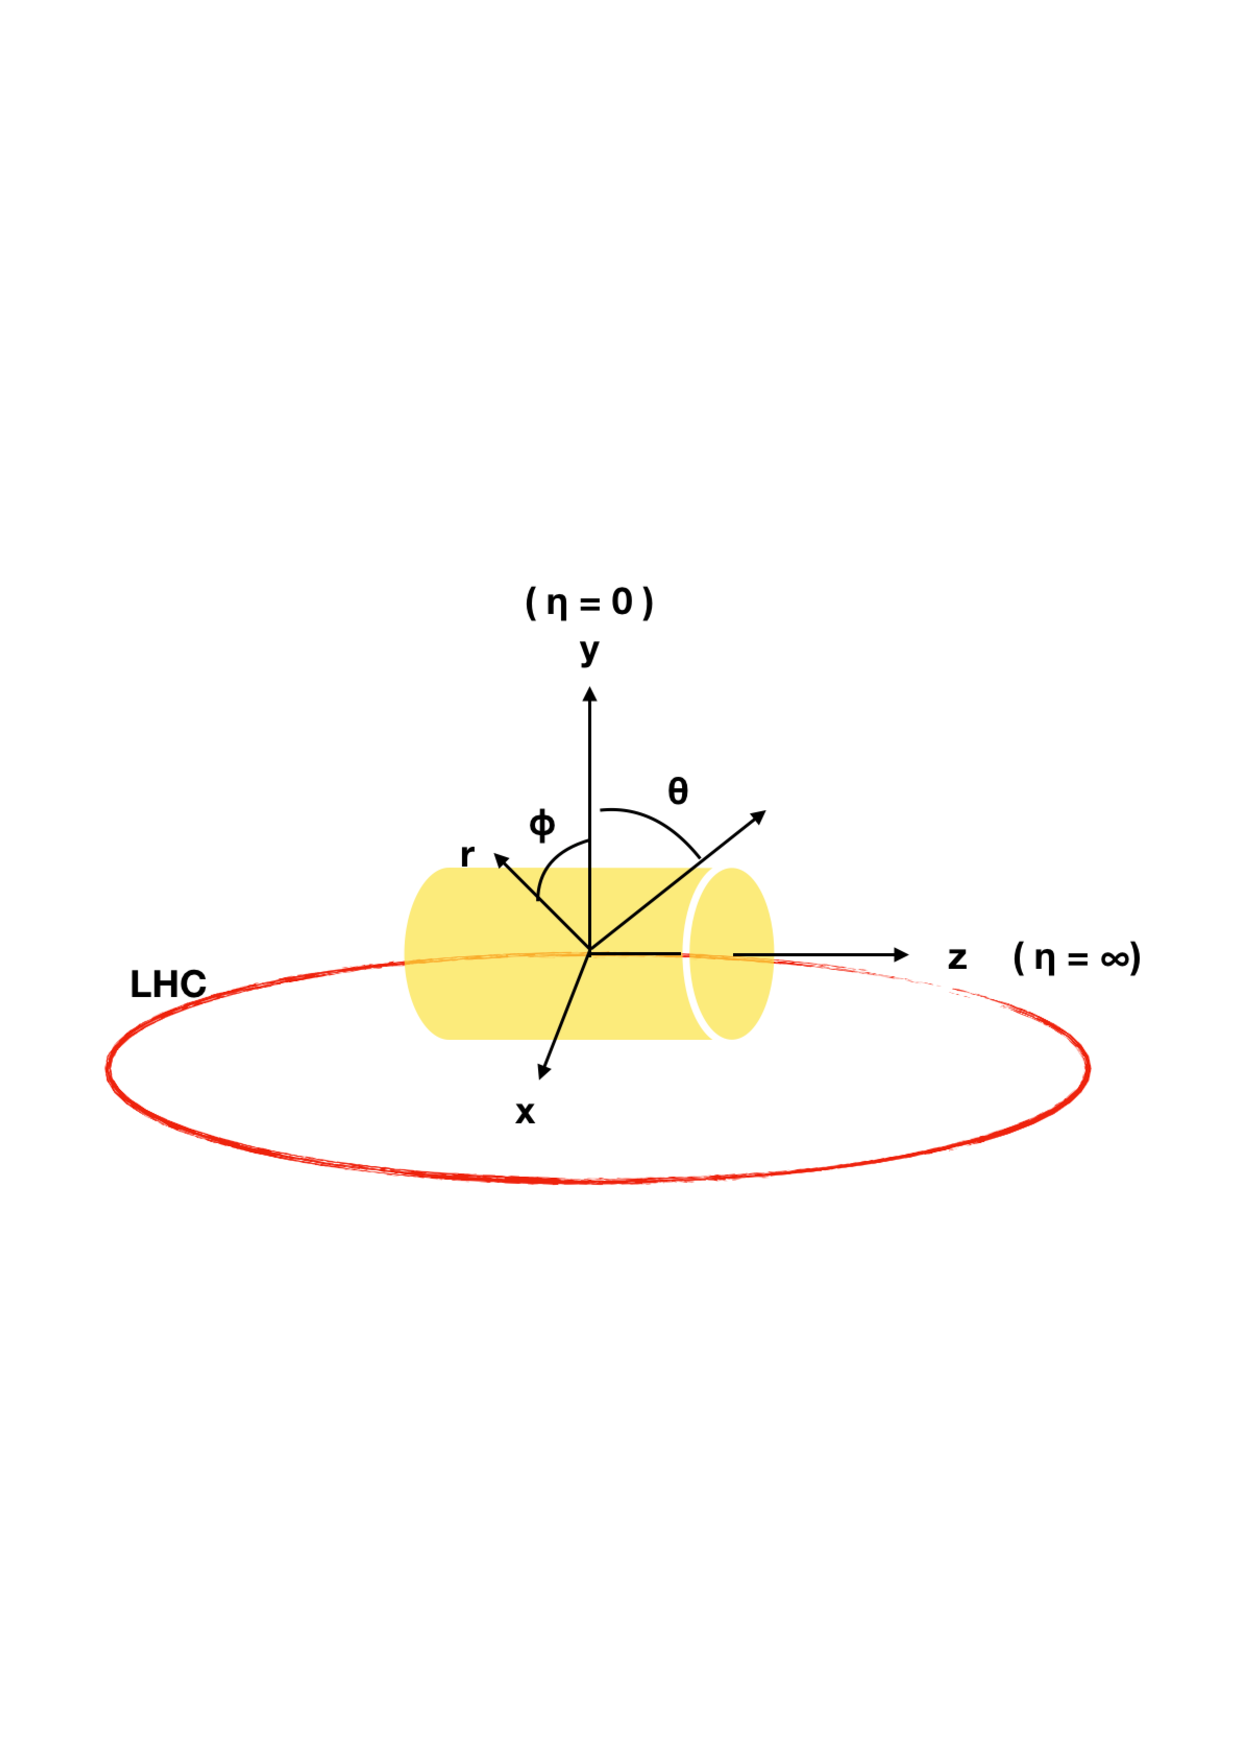
\includegraphics[width=0.65\textwidth]{figures/LHC/CMS-coordinate-system.pdf}
	\caption{The right handed coordinate system used by CMS.}
	\label{fig:cms-coordinate-system}
\end{figure}

% subsection coordinate_system (end)
%%%%%%%%%%%%%%%%%%%%%%%%%%%%%%%%%%%%%%%%%%%%%%%%%%%%%%%%%%%%%%%%%%
%%%%%%%%%%%%%%%%%%%%%%%%%%%%%%%%%%%%%%%%%%%%%%%%%%%%%%%%%%%%%%%%%%
\subsection{CMS sub-systems} % (fold)
\label{sub:cms_sub_systems}

%%%%%%%%%%%%%%%%%%%%%%%%%%%%%%%%%%%%%%%%%%%%%%%%%%%%%%%%%%%%%%%%%%
%%%%%%%%%%%%%%%%%%%%%%%%%%%%%%%%%%%%%%%%%%%%%%%%%%%%%%%%%%%%%%%%%%
\subsubsection{Magnet} % (fold)
\label{ssub:magnet}
The magnet system (see Fig.~\ref{fig:CMS-magnet}) of CMS consists of a superconducting solenoid magnet which is 12.5 m in length and has an inner diameter of 6 m. The size of the solenoid is large since the tracker, electromagnetic calorimeter and hadron calorimeter are placed inside it. In the barrel region, it generates a homogeneous magnetic field of 3.8 T. The high magnetic field ensures an appropriate bending power for the highly energetic charged particles for a precise momentum measurement. Outside the solenoid, an iron yoke is placed for the returning magnetic field. The magnetic field strength inside the iron yoke is 2 T.
\begin{figure}[!htbp]
	\centering
	\includegraphics[width=0.75\textwidth]{figures/LHC/CMS_magnet.pdf}
	\caption{CMS Magnet system~\cite{Brice2007}.}
	\label{fig:CMS-magnet}
\end{figure}

% subsubsection magnet (end)
%%%%%%%%%%%%%%%%%%%%%%%%%%%%%%%%%%%%%%%%%%%%%%%%%%%%%%%%%%%%%%%%%%
%%%%%%%%%%%%%%%%%%%%%%%%%%%%%%%%%%%%%%%%%%%%%%%%%%%%%%%%%%%%%%%%%%
\subsubsection{Tracker} % (fold)
\label{ssub:tracker}
The tracker is the first detector that encounters the particles emerging from the p-p collisions. Its purpose is to measure precisely the tracks of all charged particles crossing it. Also, it helps to reconstruct the secondary vertices to tag heavy flavour particles like b-jets or tau leptons. The particle rate is the highest in the tracker. So, it should be highly granular and response time should be fast. This condition results in a high density of on-detector electronics and this implies a large amount of material that conflicts with the aim of low material to reduce multiple scattering, bremsstrahlung, photon conversion and nuclear interactions. Thus, the type, design and number of layers of the tracker is a trade-off between the performance, the amount of material, and the cost. Considering these things in mind, the CMS collaboration decided to have first three layers of silicon pixel detector to precisely measure the primary vertex, secondary vertex and the impact parameter with a total surface area of 1 $m^2$ and 66 million pixels followed by 10 layers of  silicon micro-strip detectors covering a total area of 200 $m^2$. The tracker has a length of 5.8 m and an outer diameter 2.6 m and acceptance is up to $|\eta|<2.5$. Tracker's cross sectional view is shown in Figure~\ref{fig:tracker-cross-section}.

\begin{figure}[!htbp]
	\centering
	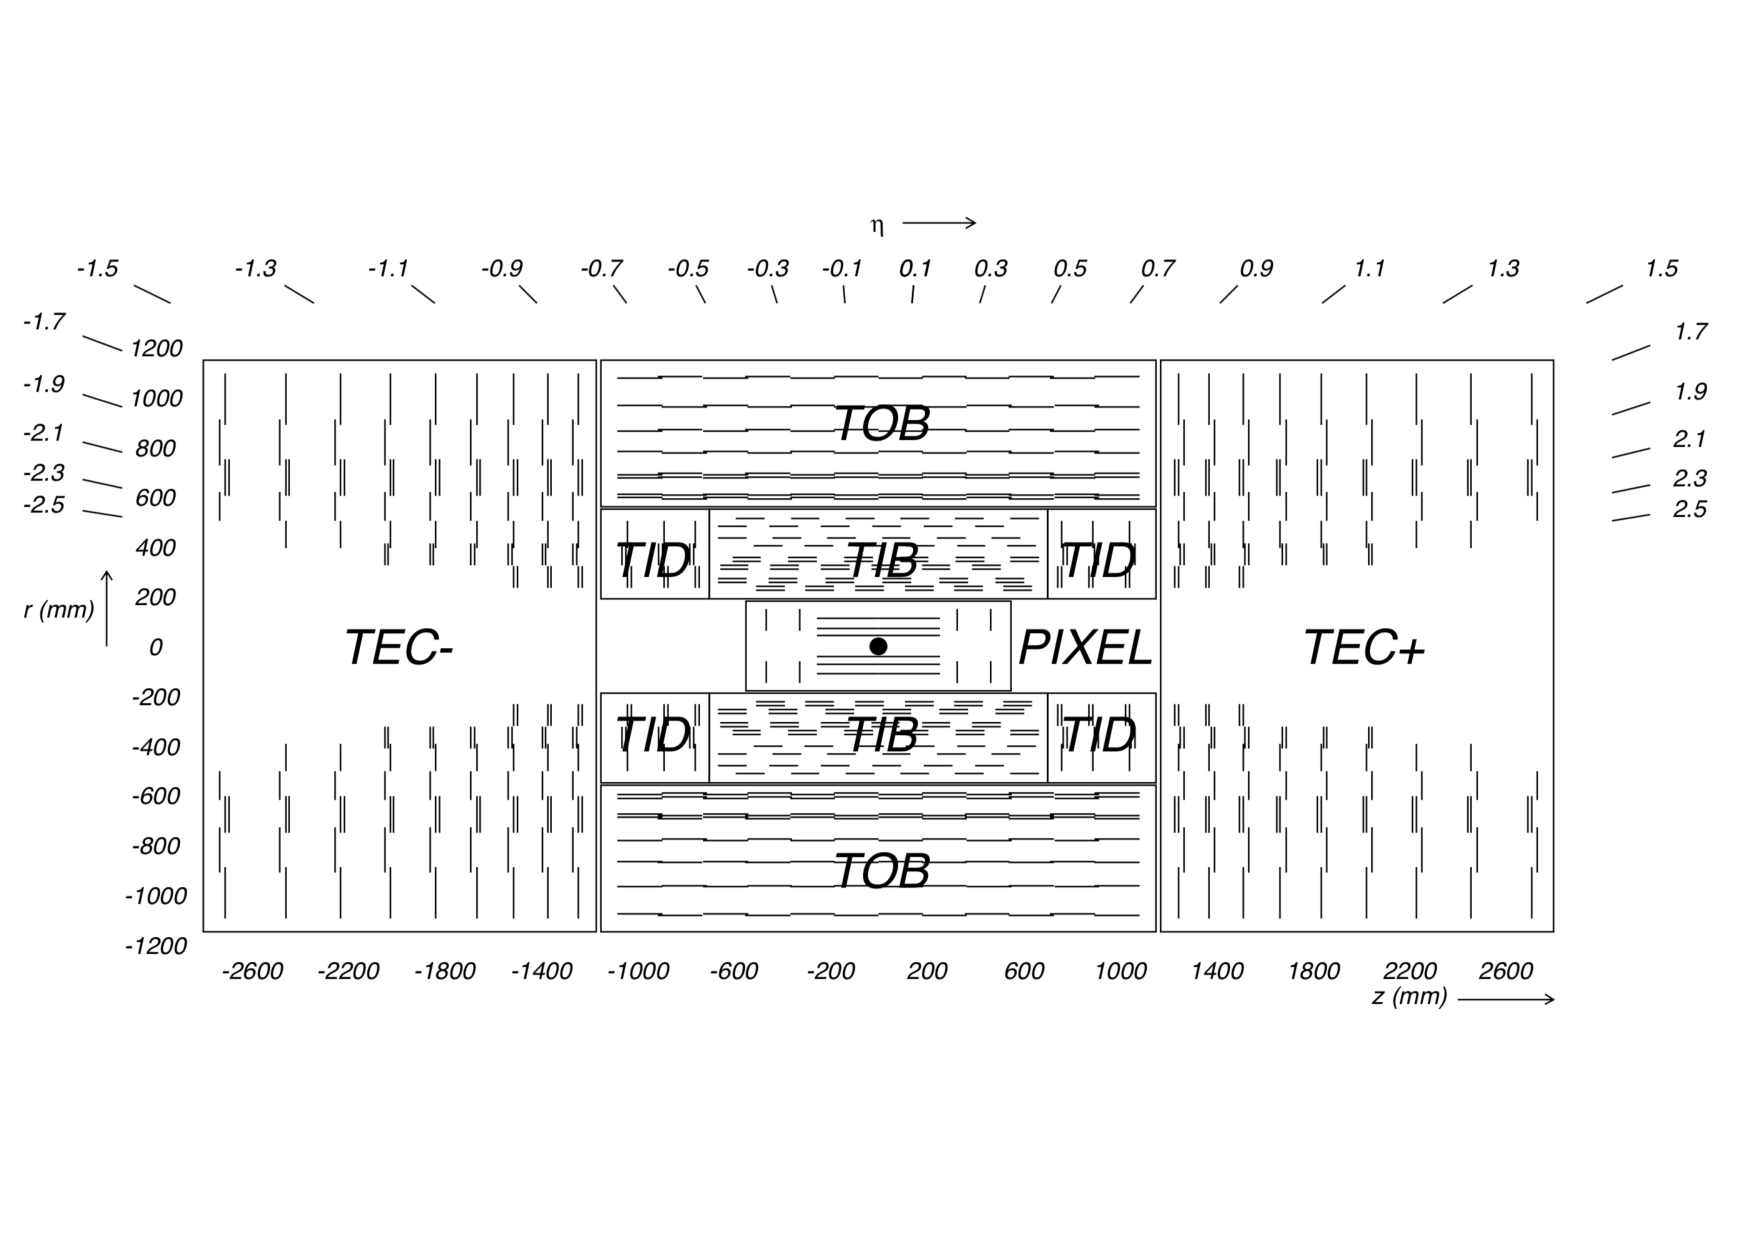
\includegraphics[width=0.95\textwidth]{figures/LHC/tracker-cross-section.pdf}
	\caption{A systematic cross section view of CMS tracker showing silicon pixel and strip detectors. Double lines show back-to-back modules that deliver stereo hits.}
	\label{fig:tracker-cross-section}
\end{figure}
% subsection tracker (end)

%%%%%%%%%%%%%%%%%%%%%%%%%%%%%%%%%%%%%%%%%%%%%%%%%%%%%%%%%%%%%%%%%%
%%%%%%%%%%%%%%%%%%%%%%%%%%%%%%%%%%%%%%%%%%%%%%%%%%%%%%%%%%%%%%%%%%

\subsubsection{Calorimetry} % (fold)
\label{ssub:calorimetry}
In general, a calorimeter is a device that measures the energy of the particles by absorption. The CMS detector uses two different types of calorimeter based on particle interactions- ECAL and HCAL. As the name suggests, the ECAL is designed to measure the particles (like electrons and photons) that primarily interacts via electromagnetic interaction while the HCAL is designed to measure particles (Hadrons, particles made up of quarks and gluons for example protons, neutrons, kaons and pions) that interact via strong nuclear interactions.\\\\
The ECAL is a homogeneous calorimeter made from lead tungstate ($PbWO_4$) crystals, having a coverage of up to $\eta < 3.0$ including a pre-shower system in the forward region. The scintillation produced in the barrel region is detected by avalanche photo-diodes and it is collected by vacuum photo-triodes in the endcaps. In terms of radiation length\footnote{Radiation length is defined as the mean length travelled by the particle to reduce its energy by a factor of 1/e.}, $X_0$, its thickness is 25$X_0$ which guarantees almost full shower containment.\\\\
In between ECAL and magnet system, the brass/scintillator sampling HCAL with coverage up to $\eta < 3.0$ is placed. To have a full geometric coverage it extends up to $\eta < 5.0$ using forward sampling iron/quartz-fibre calorimeter. This is crucial to measure the (missing) transverse energy of the event.

% The energy resolution of the ECAL can be parameterized  
% subsubsection calorimetry (end)


%%%%%%%%%%%%%%%%%%%%%%%%%%%%%%%%%%%%%%%%%%%%%%%%%%%%%%%%%%%%%%%%%%
%%%%%%%%%%%%%%%%%%%%%%%%%%%%%%%%%%%%%%%%%%%%%%%%%%%%%%%%%%%%%%%%%%
\subsubsection{The Muon System} % (fold)
\label{sub:the_muon_system}
It is evident  from the name of the CMS detector that a precise detection of muons is one of its main targets. It is motivated by the presence of muons in the final state of many interesting physics processes, such as the decay of Higgs boson into ZZ which subsequently decays into four leptons and especially, the case where all four leptons are muons, are referred to as the ``gold plated'' channel as we can detect muons efficiently over higher background contributions at LHC. At CMS, the muon system serves three different functions viz. identification, momentum measurement and triggering of muons. The strong superconducting magnet system with its return yoke of CMS, helps to acquire good momentum measurement and triggering capabilities. The return yoke of magnet system also serves as the hadron absorber. Only muons leave their tracks in the muon detector system, as all other particles are already absorbed by the calorimeters. Thus, the appearance of charged particle in the muon system signifies that it can only be from muon. The track left by muon in the CMS detector is illustrated in Figure~\ref{fig:muon-system-cross}. 
\begin{figure}[!htbp]
	\centering
	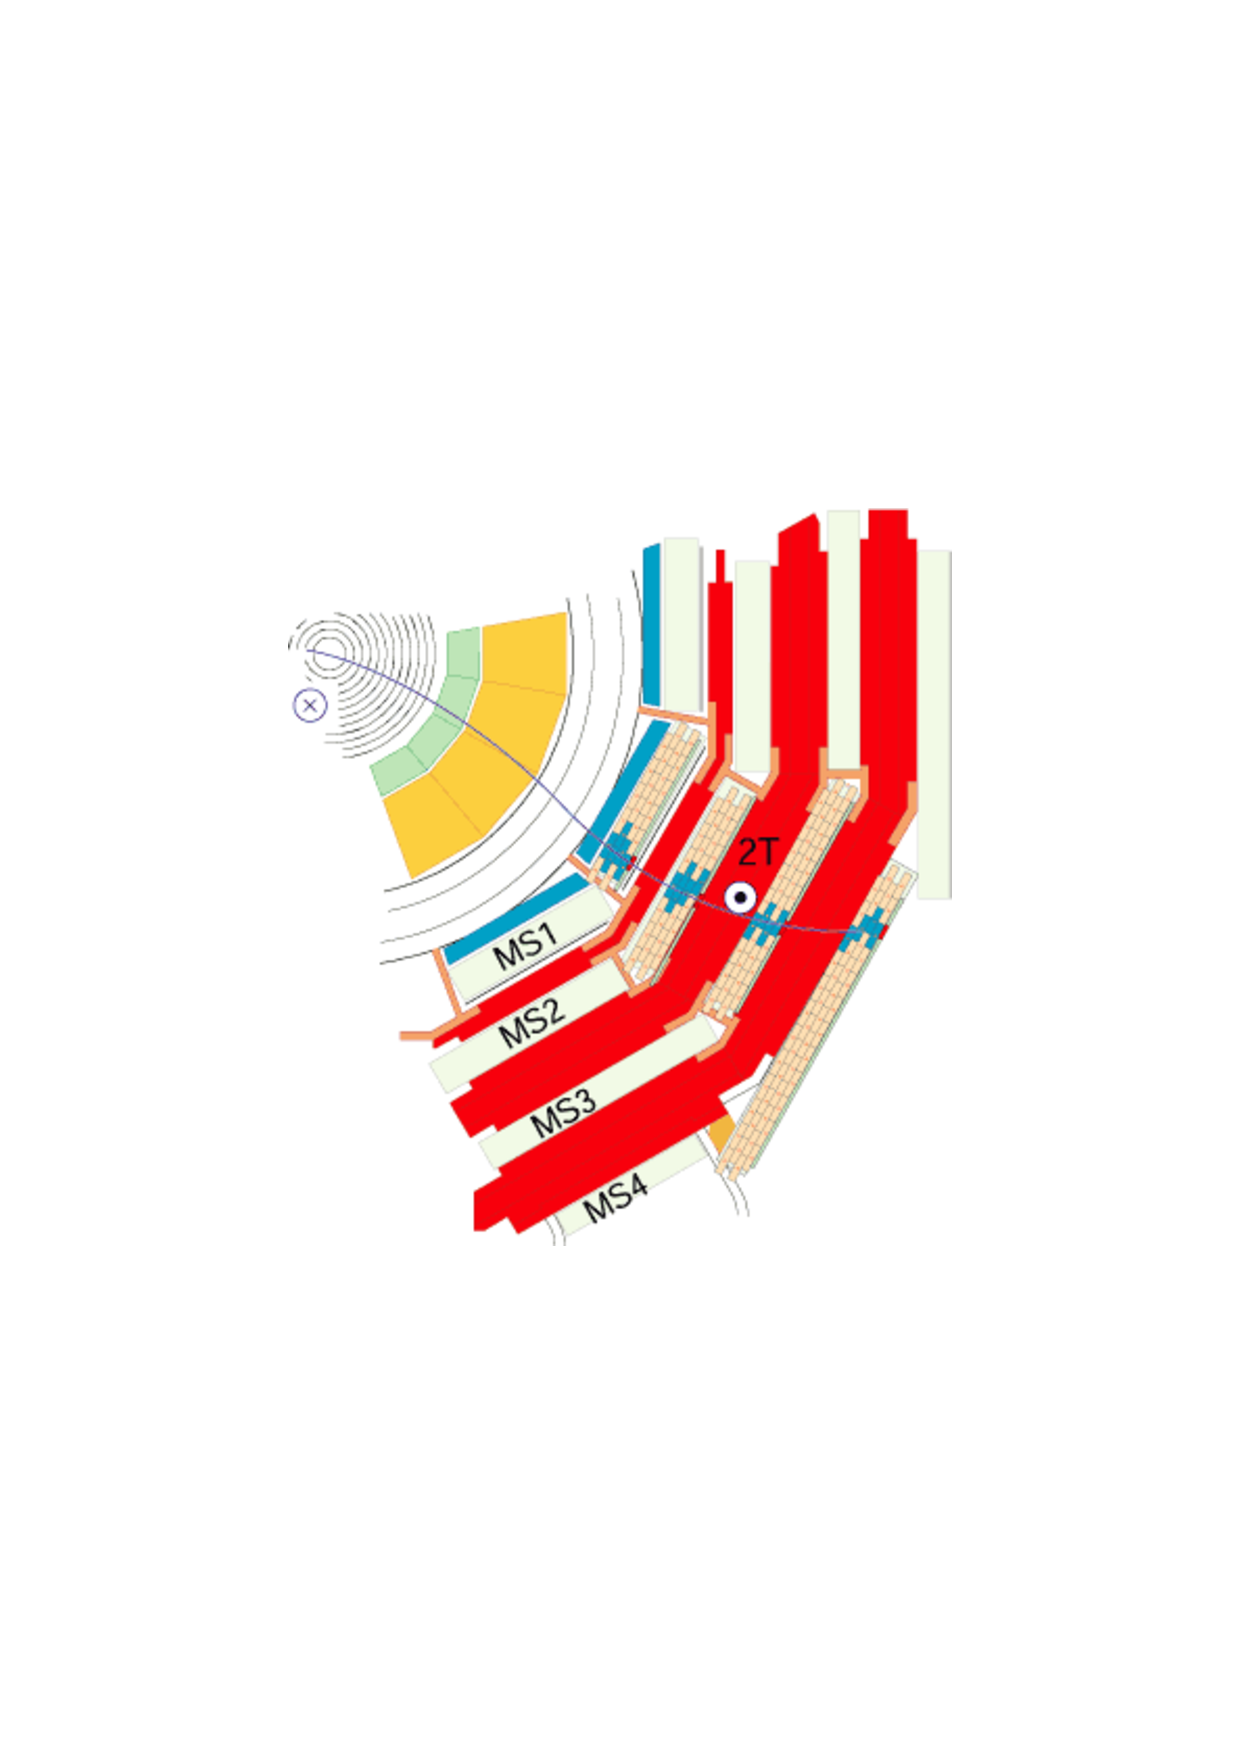
\includegraphics[width=0.45\textwidth]{figures/LHC/MuStations.pdf}
	\caption{A muon leaves curved trajectory in LHC and the bending changes as the magnetic field direction of solenoid inside and outside are opposite.}
	\label{fig:muon-system-cross}
\end{figure}
The layout of the CMS muon detector system is shown in Figure~\ref{fig:muon-system-layout}.
Three different types of gaseous detectors used for the muon system  were chosen based on the background level, muon rate, uniformity and magnitude of magnetic field.
Drift tubes (DT) are used as tracking detector in the barrel region with relatively lower magnetic field intensity and have lower background rates as compared to the endcaps. 
For the endcap regions, Cathode Strip Chambers (CSC) are employed as they provide precise information about muons momentum and timing information even under high radiation environment.
The pseudo-rapidity coverage of DTs is $|\eta|<1.2$ and for CSCs is $0.9<|\eta|<2.4$. Along with DTs and CSCs, Resistive Plate Chamber (RPC) detectors are also installed to have a fast dedicated  muon triggering system in both barrel and endcap region up to $|\eta|<1.6$~\cite{muon-tdr}. The CMS muon detector system covers the geometric region up to $|\eta|<2.4$ but RPCs are deployed up-to $|\eta|<1.6$ as RPCs cannot withstand the radiation level after pseudo-rapidity region of 1.6. Thus to reconstruct muons in pseudo-rapidity region higher than 1.6 during Long Shutdown-2 (LS2, 2019-2020), CMS collaboration decided to employ Gas Electron Multiplier (GEM) detectors in region  $1.6<|\eta|<2.2$, which is able to provide good space resolution and time resolution even in high environment radiation. The pseudo-rapidity range is limited to $|\eta|<2.2$ because of space constrains. GEM  detectors are described in details in Chapter~\ref{cha:gas_electron_multiplier}.
\begin{figure}[!htbp]
	% \vspace{-3.2em}
	\centering
	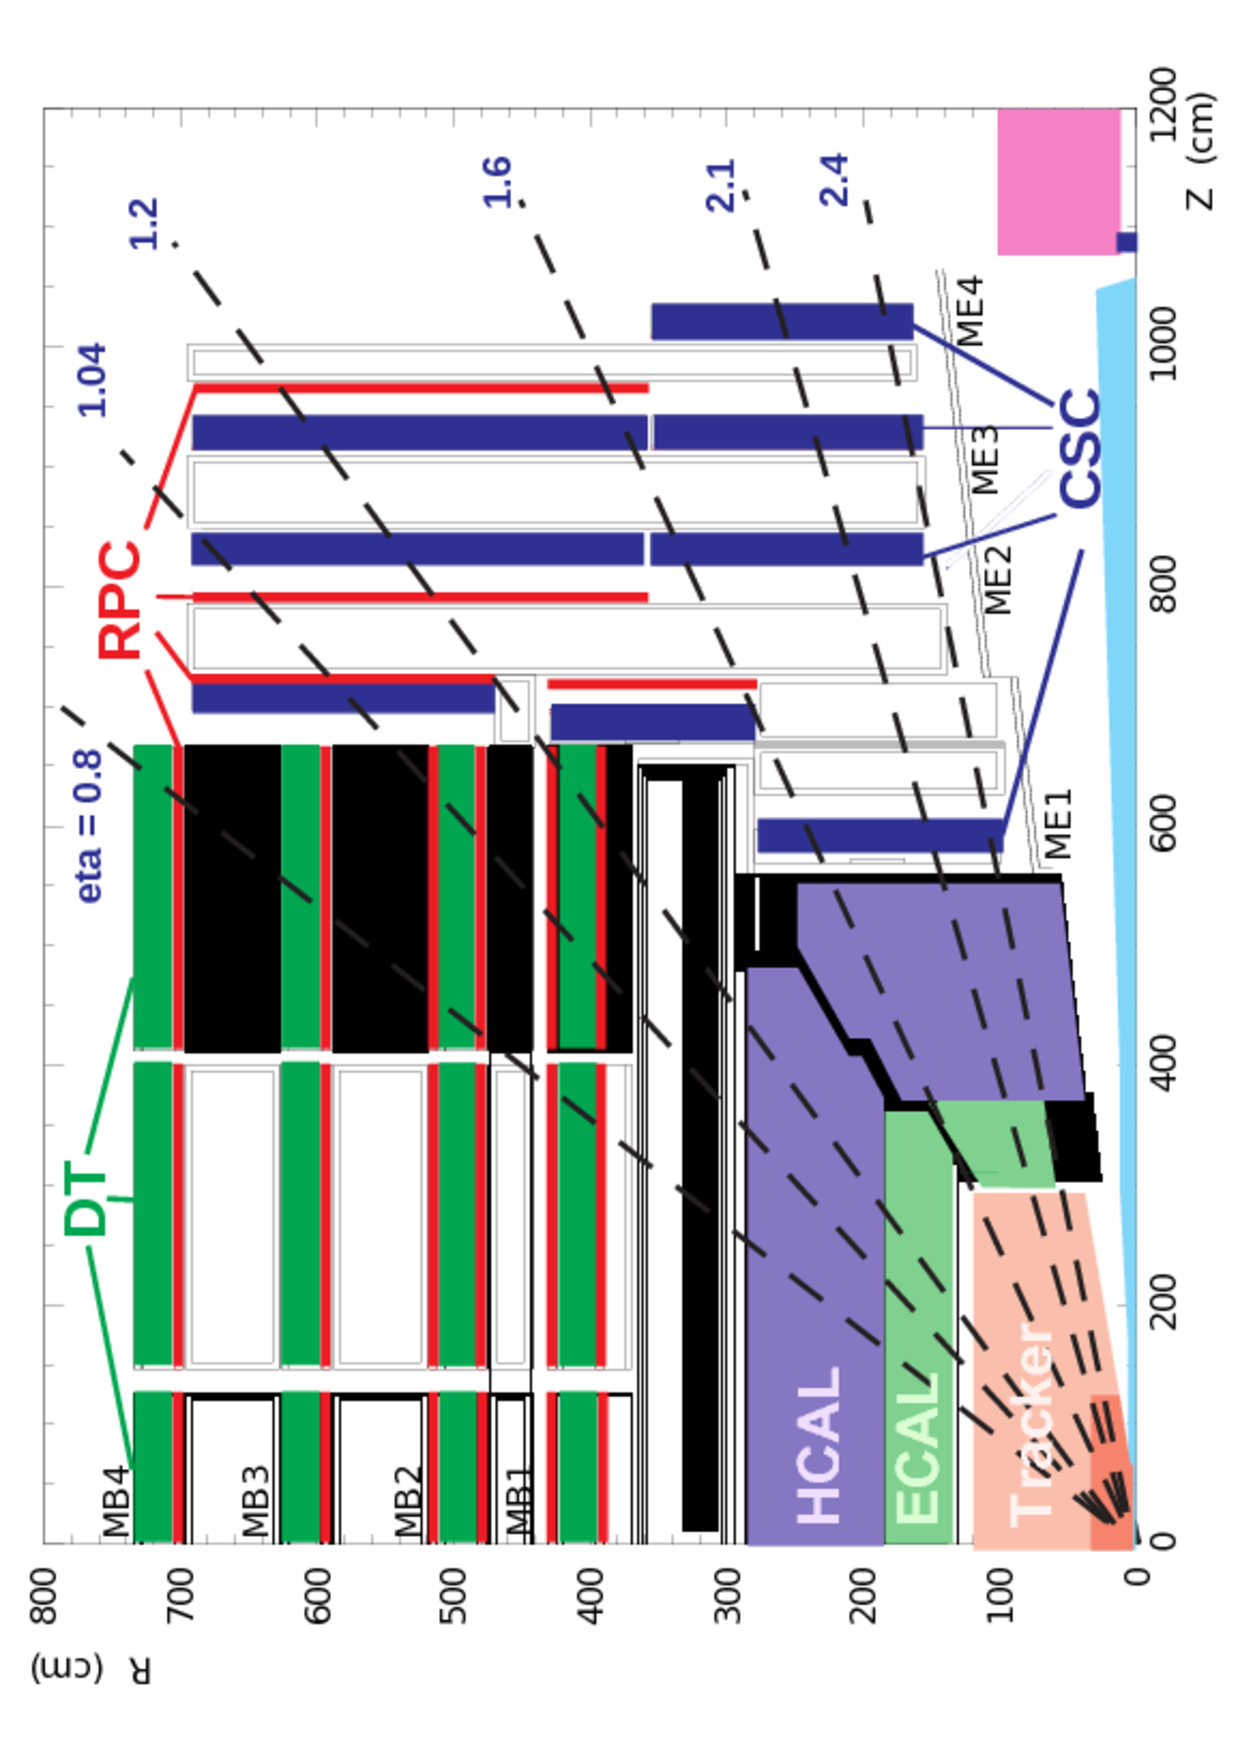
\includegraphics[width=0.75\textwidth]{figures/LHC/pictures_MuonSys-mod3.pdf}
	\caption{Longitudinal layout of one quadrant of the CMS detector. There are four DT stations named MB1-MB4 marked with green colour. Four CMS systems in high pseudo-rapidity region named ME1-ME4 in blue colour. Also, there are several RPC stations in barrel region and part of endcap region marked with red colour.}
	\label{fig:muon-system-layout}
\end{figure}
Summary of CMS detector sub-system including its main characteristics and composition is given in Table~\ref{table:CMSMainChar}.
% subsection the_muon_system (end)
% subsection cms_sub_systems (end)
% % section cms_experiment (end)

\begin{table}
% \vspace{-5.2em}
\centering
\begin{tabular}[!htbp]{l l l}
\hline
{\textbf{Sub-system}} & {\textbf{Composition}} & {\textbf{Charateristics}} \\
\hline
Tracker  & Silicon strip and  & isolated track efficiency $\epsilon > 95\%$ \\
	& pixel detector	& within jets $\epsilon \sim 90\%$ \\
	& 	& primary vertex resolution: 10-20 $\mu m$ \\
	& 	& $p_T$ resolution: $\Delta p_T/p_T = 1\%$ (0.1 TeV), 10\% (TeV)\\
	& 	& coverage $\eta<2.4$ \\
\hline
ECAL 	& 	$PbWO_4$ crystals 	& energy resolution:\\
		& 	& $\big(\frac{\sigma}{E}\big)^2 = \big(\frac{2.7\%}{\sqrt{E}}\big)^2 + \big(\frac{210}{E}\big)^2 + 0.55\% $  (barrel)\\
		& 	& $\big(\frac{\sigma}{E}\big)^2 = \big(\frac{5.7\%}{\sqrt{E}}\big)^2 + \big(\frac{245}{E}\big)^2 + 0.55\% $  (end-caps)\\
		& 	& coverage $\eta < 3$ \\
\hline
HCAL 	& 	Cu-Zn 	& energy resolution:\\
		& 	scintillator & $\big(\frac{\sigma}{E}\big)^2 = \big(\frac{68\%}{\sqrt{E}}\big)^2 + 4.5\%$ \\
		& 	& coverage $\eta < 3$ \\
\hline
Muon system & Gaseous & efficiency $\epsilon \sim 98\%$ \\
			& detectors & $\Delta p_T/p_T =$8-15 \% (0.01 TeV)/20-40\% (TeV)\\
		& 	& coverage $\eta < 2.4$ \\
\hline
\end{tabular}
\caption{Main characteristics of the CMS sub-system~\cite{JeremieThesis}}
\label{table:CMSMainChar}
\end{table}


% % %%%%%%%%%%%%%%%%%%%%%%%%%%%%%%%%%%%%%%%%%%%%%%%%%%%%%%%%%%%%%%%%%%
\subsection{CMS Trigger and Data Acquisition system} % (fold)
\label{sub:cms_trigger_and_data_acquisition_system}
The LHC produces about 1 billion of p-p collisions every second.
During each collision thousands of particles are produced that cross the CMS detector.
Reconstruction of all these particles generate several Terabytes of data.
However, till date we neither have a switch with the required bandwidth that can transfer this enormous data for further processing nor the disk space to store all of them.
Though if we have one, only a few fractions of data that are interesting for new physics or help us to understand the existing one as most of the collisions are the low-energy glancing collisions instead of head-on interaction.
Also, this can be understood from the SM cross-section of pp as compared to the other process shown in Fig.~\ref{fig:SM-cross-section}.
\begin{figure}[!htbp]
	\centering
	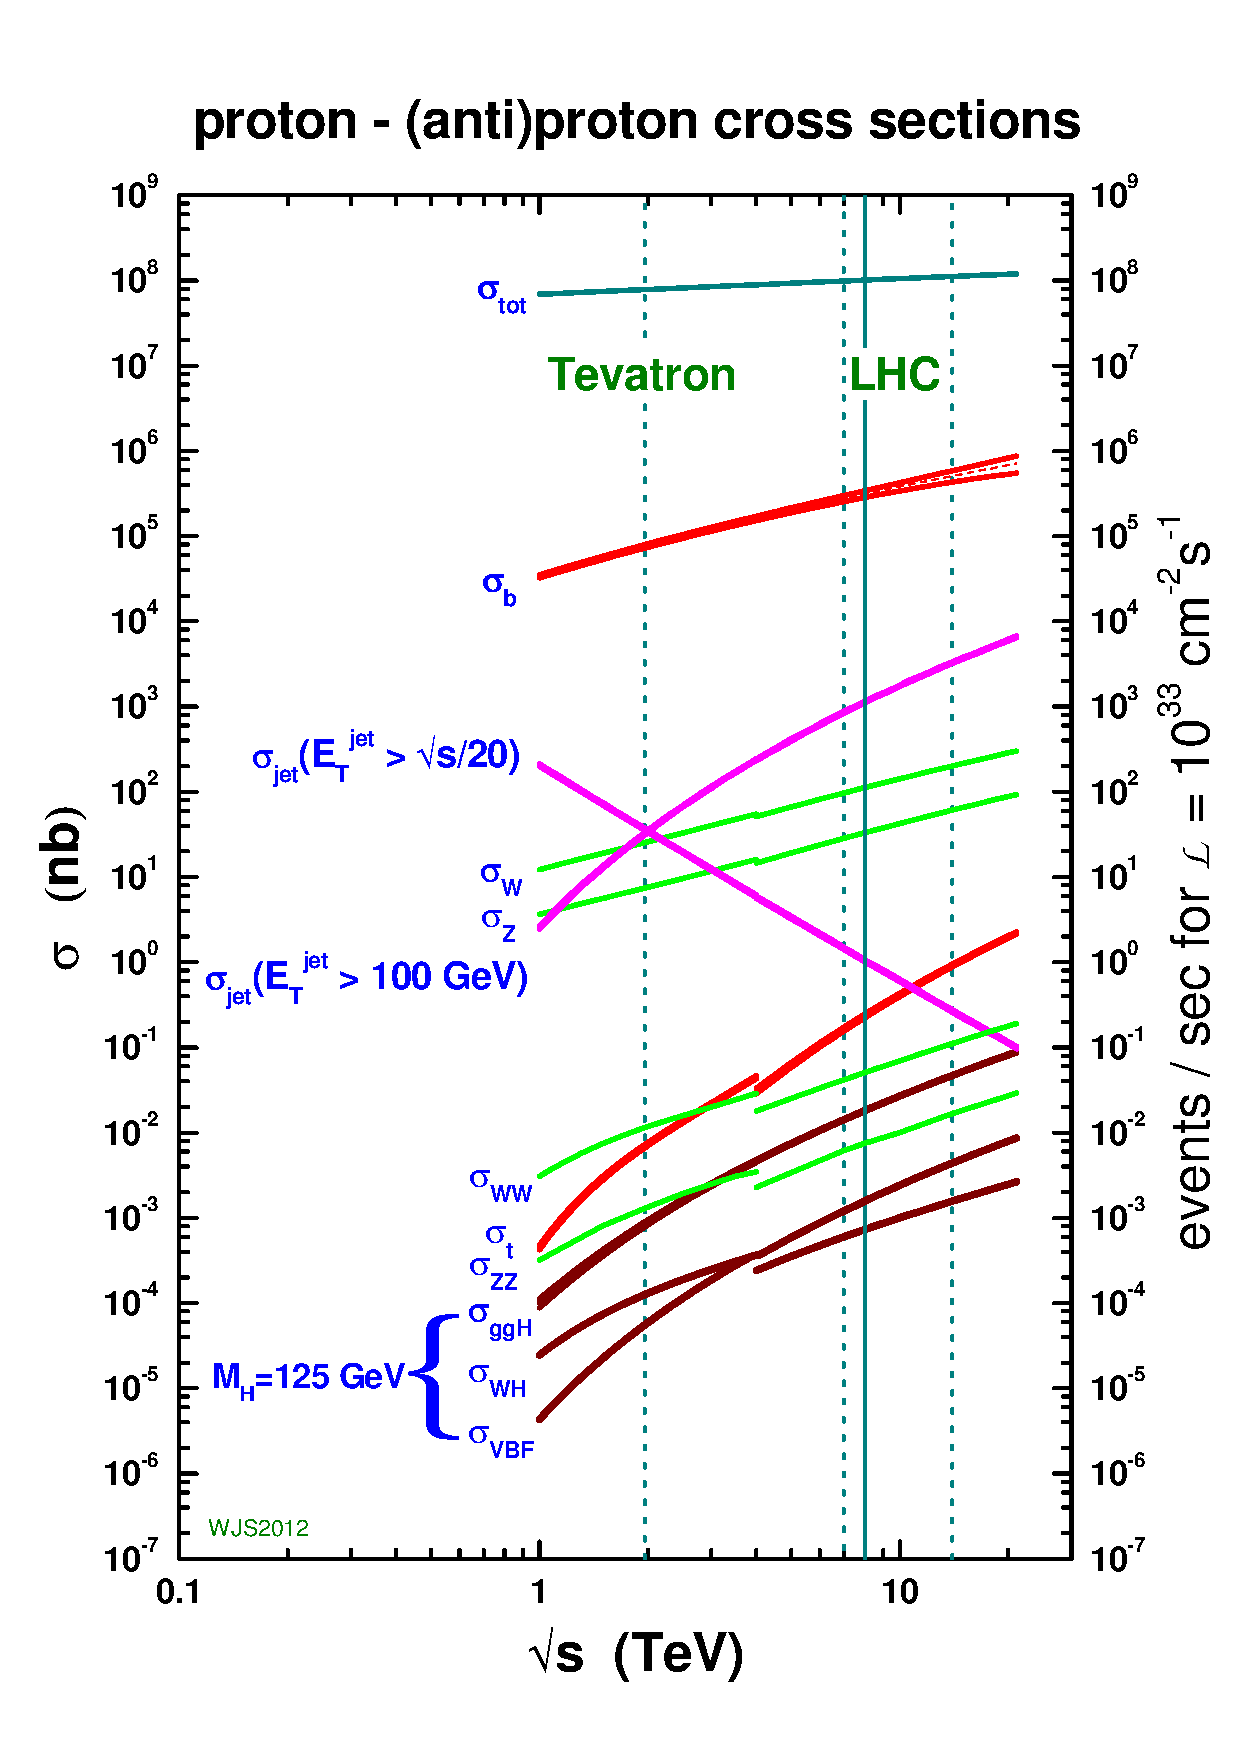
\includegraphics[width=0.65\textwidth]{figures/LHC/crosssections2012_v5.pdf}
	\caption{Standard Model cross sections as a function of collider energy~\cite{Stirling2012}. The total hadronic cross-section is based on parametrisation of the Particle Data Group~\cite{PDG2018}. Other cross-sections are calculated at NLO or NNLO perturbative QCD, using MSTW2008 parton distributions~\cite{Martin2009}.}
	\label{fig:SM-cross-section}
\end{figure}
The maximum amount of data that can be stored every day is of the order of few Terabytes that decide the rate at which we can accept the events ($\sim$ 100 Hz).
Thus, the concept of the trigger, method to select events of interest, was first introduced by ZEUS experiment~\cite{ZEUSCollaboration1993}, that handles data in real time, coupled with complex data acquisition (DAQ) system.
While designing the trigger one has to keep in mind that trigger should efficiently accept the interesting physics while rejecting the non-interesting ones as whatever information is lost at this level can not be recovered.

The CMS trigger system is divided into two steps - Level-1 trigger which is a custom hardware running synchronously with the LHC bunch crossing frequency of 40 MHz and the High-Level Trigger (HLT)~\cite{paper:JINST:CMSCollaboration,Cittolin:578006,Khachatryan2017}. The CMS trigger flow diagram is shown in Fig.~\ref{fig:cms-trigger}. 
\begin{figure}[!htbp]
	\centering
	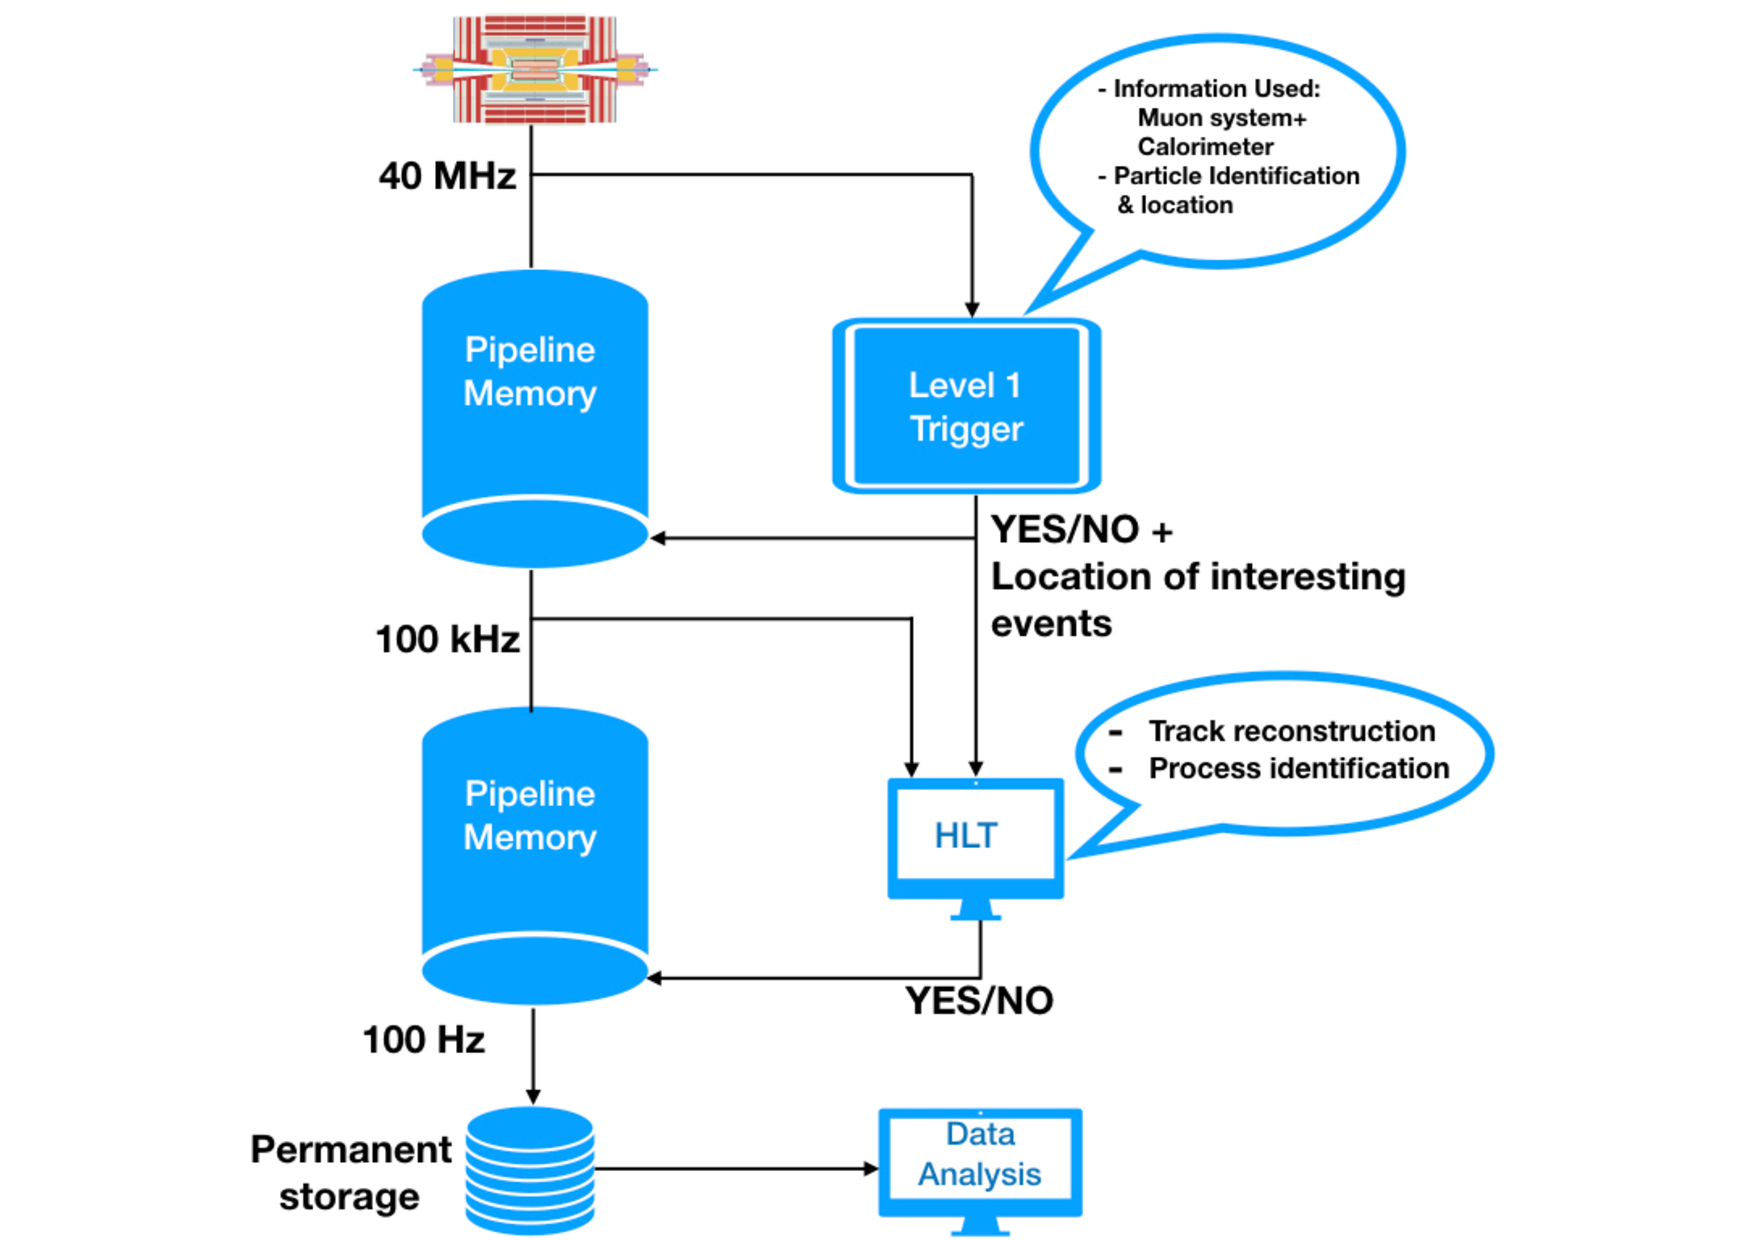
\includegraphics[width=0.9\textwidth,height=0.63\textwidth]{figures/LHC/Trigger-flow-diagram.pdf}
	\caption{CMS trigger flow diagram that uses two level trigger. At Level 1, CMS uses information from muon system and calorimeter. Using this information it decides to reject  or pass the event to the HLT farm for further processing. HLT uses fast offline reconstruction algorithm that uses information from all sub-system, i.e., calorimeters, muon system as well as tracker to decide to keep or reject the event.}
	\label{fig:cms-trigger}
\end{figure}

\subsubsection{Level-1 Trigger} % (fold)
\label{ssub:level_1_trigger}
The Level-1 trigger checks each event and decides if they can go for further scrutiny by the HLT.
It analyses each event based on the coarser level granularity information of calorimeter (both ECAL and HCAL) and tracks from muon system.
However, this decision cannot take place within 25 ns (i.e. before arrival of next p-p bunch crossing), so a latency\footnote{The latency is the time elapsed between a pp interaction and the arrival of the Level-1 trigger decision at the Front-End. The Front-End system processes and keeps all detector signals in buffer until they are delivered to the Data Acquisition System (DAQ)} of 3.2 $\mu s$ was added, which is named as pipeline memory in Fig.~\ref{fig:cms-trigger}.
At Level-1 the event reduces rate from 40MHz to 100kHz.

The Level-1 consists of three steps. They are:
\begin{itemize}
	\item Level-1 calorimeter trigger,
	\item Level-1 muon trigger,
	\item Level-1 global trigger
\end{itemize}
Every step at Level-1 trigger has local, regional and global components. At first the local components, which is also called Trigger Primitive Generators (TPG), are based on the energy deposit in the calorimeter trigger towers\footnote{Trigger towers are the arrays of crystals where energy is deposited.} and track segments or hit patterns in the muon chambers, respectively. 
Next, the regional trigger combines this information to identify the pattern logic and determine ranked and sorted objects such as electrons, photons, or muons. Finally, the global component determines the highest-ranked objects across the detectors and transfer it to the Level-1 global trigger. The flow diagram of Level-1 trigger is shown in Fig.~\ref{fig:cms-L1-trigger}.
\begin{figure}[htbp]
	\centering
	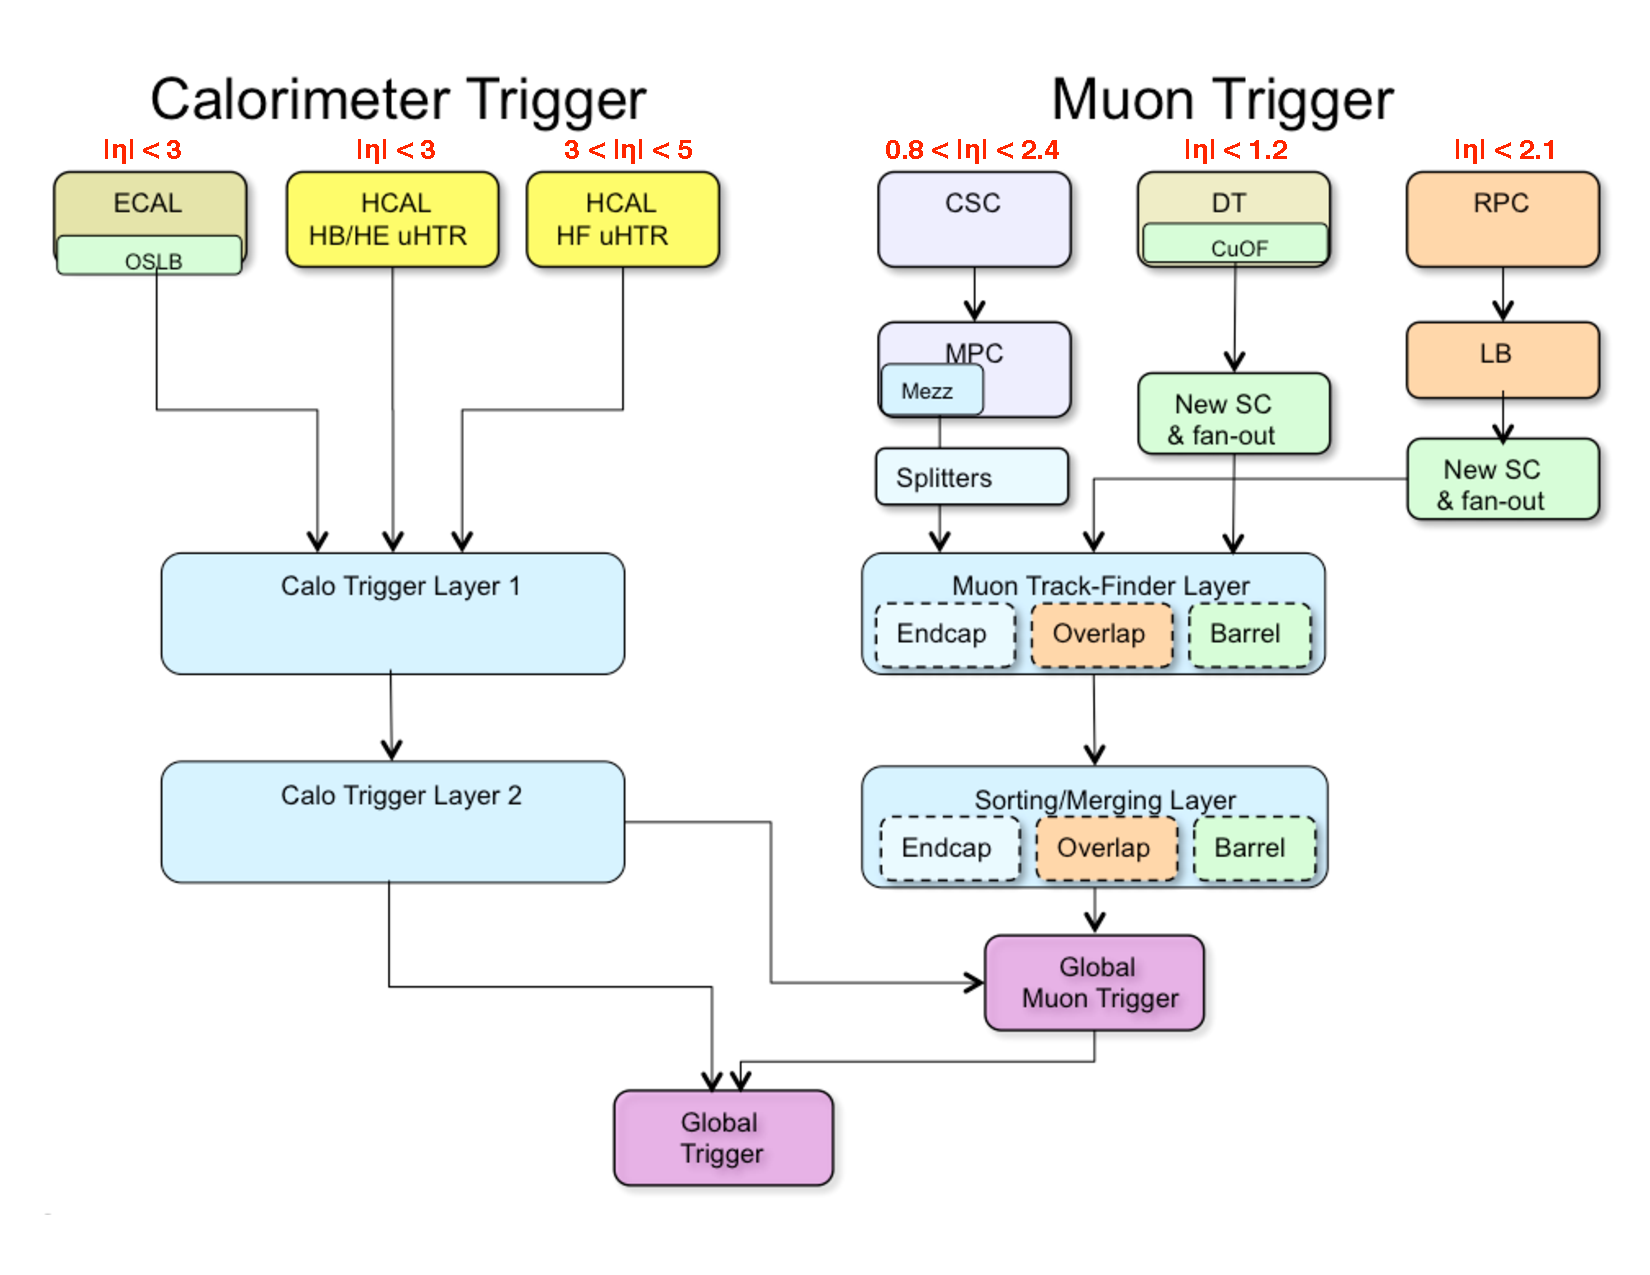
\includegraphics[width=0.7\textwidth]{figures/LHC/TriggerBlockDiagram_Eta.pdf}
	\caption{CMS Level-1 trigger flow diagram~\cite{L1trigger-2013}. On left the hierarchy of calorimeter trigger is shown. On right the different layers of the muon trigger system is shown. Finally the global trigger combines information from both system to take the Level-1 decision.}
	\label{fig:cms-L1-trigger}
\end{figure}

\subsubsection{Level-1 Calorimeter Trigger} % (fold)
\label{ssub:l1_calorimeter_trigger}
The first step of calorimeter trigger is TPG. The TPG is the sum of transverse energy measured in ECAL crystals or HCAL readout towers to obtain trigger towers and it also attaches bunch crossing information with this. Information in the form of TPG is transferred to the Regional Calorimeter Trigger (RCT). Then the information from RCT is combined to the Global Calorimeter Trigger (GCT) where the best four candidates in each category are chosen and sent to the global trigger.

% subsubsection l1_calorimeter_trigger (end)


\subsubsection{Level-1 Muon Trigger} % (fold)
\label{ssub:l1_muon_trigger}
In Level-1 muon trigger, all three muon systems, i.e. DT, CSC and RPC, take part. Considering the difference in particle flux and the magnetic field uniformity with $\eta$ the muon track finding was segmented into three regions: Barrel ($|\eta|<0.83$), Overlap ($0.83<|\eta| < 1.24$) and Endcap ($|\eta|>1.24$). A pattern based track finding algorithm~\cite{Eroe2008} is used at endcap and overlap region. It assigns $p_T$ to each track using the look-up-table based on multivariate techniques. In barrel region a simple extrapolation track finding algorithm is used. Finally, the Level-1 global muon trigger takes all the muons from three different muon sub-detectors regional track finders, then sorts and ranks them using their $p_T$ value and quality.

% subsubsection l1_muon_trigger (end)

\subsubsection{Level-1 Global Trigger} % (fold)
\label{ssub:l1_global_trigger}
The Level-1 global trigger takes input from Level-1 calorimeter and  muon triggers. Also, it aligns them in time and  decides to accept or reject an event. Additionally, a direct trigger signal is also received from the sub-detectors or the TOTEM experiment for some special purpose such as calibration. These received trigger signal to the level 1 global trigger are known as ``technical triggers''. 

The main part of the global trigger is known as the ``Global Trigger Logic'' board, where all the implemented algorithm are performed. The most basic algorithm consists of applying the transverse momentum ($p_T$) or the transverse energy ($E_T$) or the jet multiplicity which exceeding the required cut. Finally the passed events are sent to the data acquisition event manager for further processing by HLT.

% subsubsection l1_global_trigger (end)

% subsubsection level_1_trigger (end)

\subsubsection{High Level Trigger} % (fold)
\label{ssub:high_level_trigger}
The complete information of the passed events by Level-1 trigger is sent to HLT processing farm to reduce the event rate to $\sim$100 Hz. HLT algorithm runs on commercial computer that have about 16,000 CPU cores and performs fast version of offline object reconstruction using the information from all sub-detectors. 

In CMS, the HLT has a modular structure, which is shown in Fig.~\ref{fig:HLT_menue_workflow}.
\begin{figure}[htbp]
	\centering
	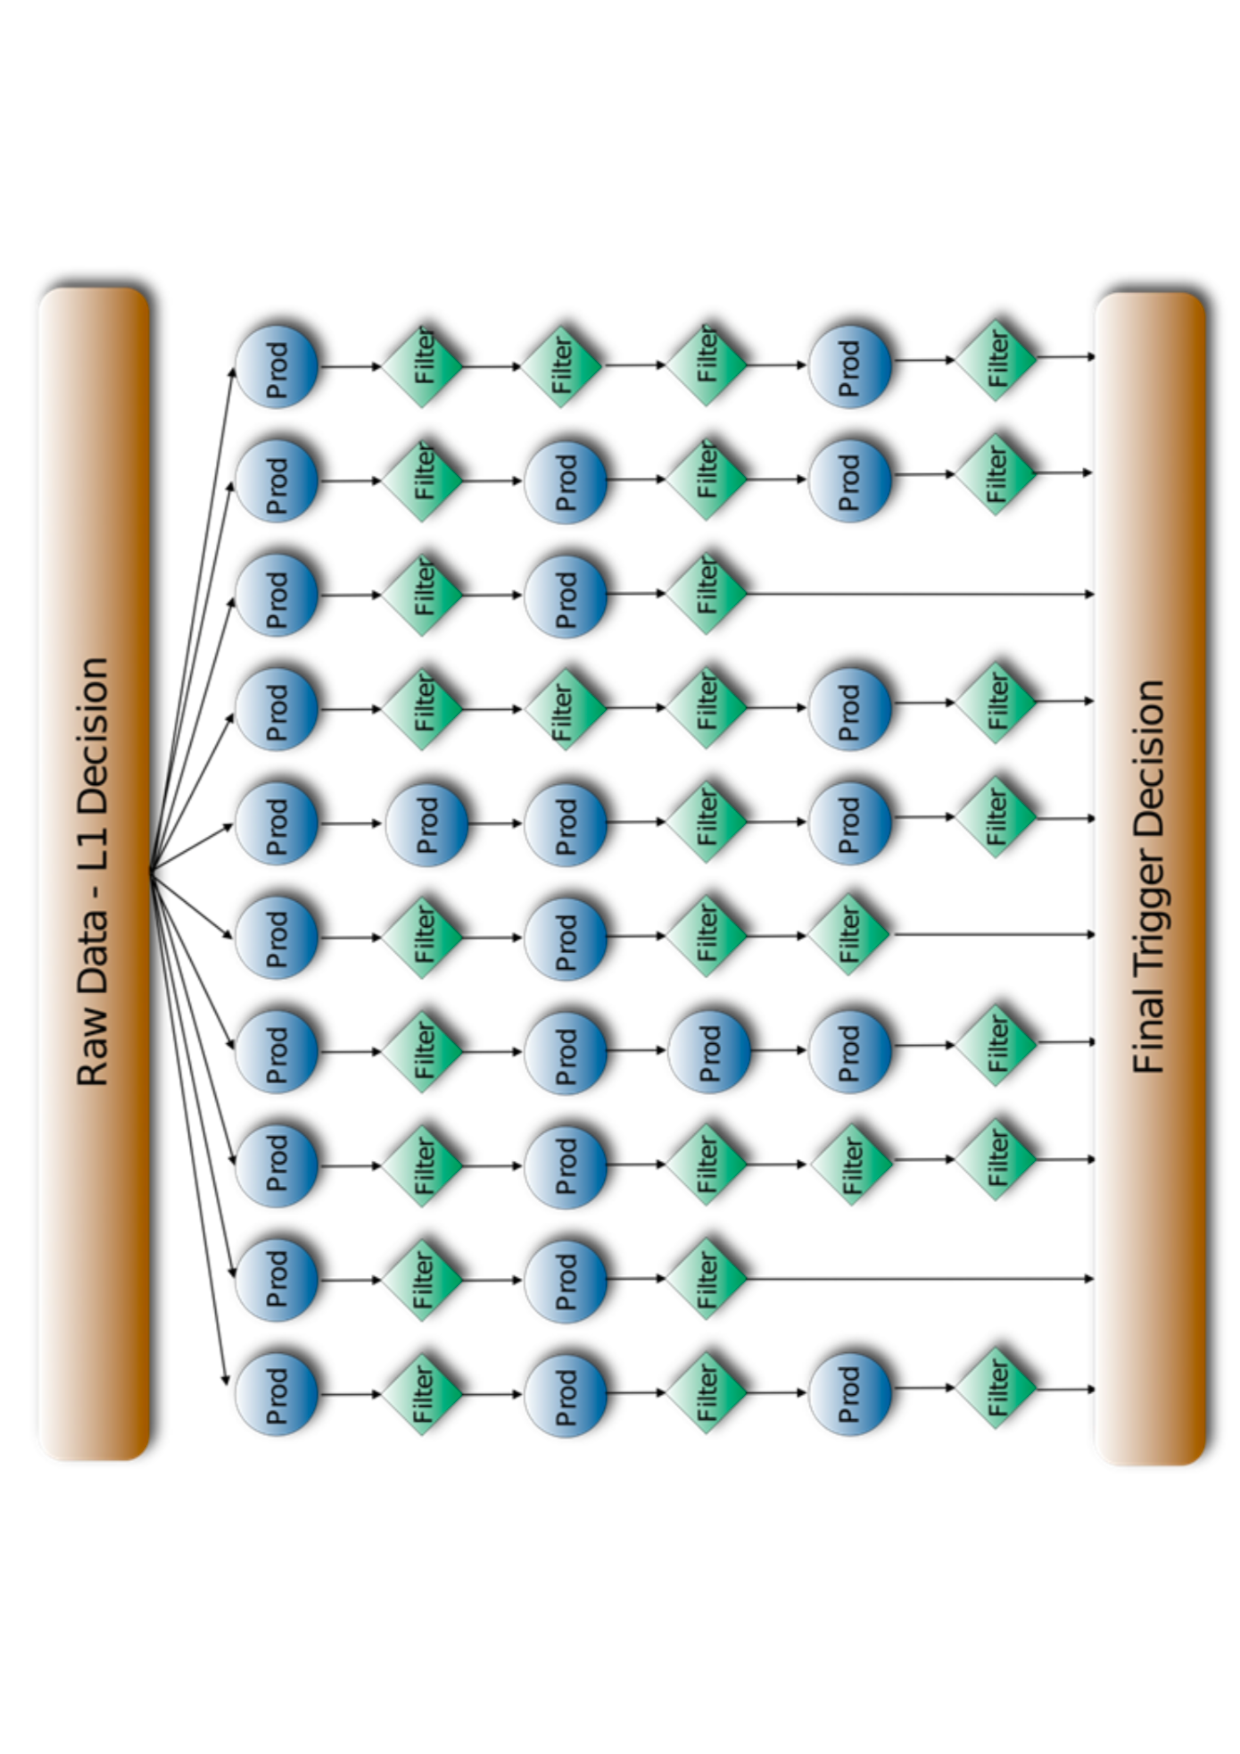
\includegraphics[width=0.65\textwidth]{figures/LHC/HLT_menu_workflow.pdf}
	\caption{The systematic representation of HLT menu and its path\cite{Perrotta2015}.}
	\label{fig:HLT_menue_workflow}
\end{figure}
The HLT menu is made up of many HLT paths. There are around 400 different HLT paths in the HLT menu for the data taken during Run2. Example of several trigger paths is given in Table:~\ref{tab:trigger-path}. Each path consists of a sequence of reconstruction and filtering modules.  The modules in each path are either object producers or filters. The producer modules reconstruct the object like electron, photon,  muons, jets and their properties. Filter module take decision using the variables reconstructed by producer modules to accept or reject an event. All the producers and filters are arranged in blocks in order of their complexity, so that faster algorithm runs first and their products are filtered. If a filter fails the rest of path skips. At last the final decision is the logical OR of all the HLT menu decisions.
% To restrict table inside the page
% Reference: https://tex.stackexchange.com/a/245384/41568
\begin{table}
{\small
\begin{tabular}[!htbp]{l p{0.55\linewidth}}
\hline
{\textbf{Trigger Path}} & {\textbf{Explanation}} \\
\hline
HLT\_Ele27\_WPTight\_Gsf\_v7 & Requires at least one electron at the HLT level having $p_T$ greater than 27 GeV along with some tight selection criteria on its kinematic variables. The electron is reconstructed using the Gaussian Sum Filter (GSF) technique\footnote{In CMS detector we use large amount of material that includes detector itself along with the on detector electronics, mechanical support and power cooling. Thus along with the ionization energy loss and multiple coulomb scattering it also suffers from energy loss due to bremsstrahlung. Thus, to  precisely model the track, we have to include the material effects. This is done using the linear generalization of Kalman Filter\cite{Kalman1960}, the GSF\cite{Fruehwirth1998,Fruehwirth1997} in the track reconstruction. It assumes all the different components of different degrees of the bremsstrahlung under consideration as the sum of several Gaussian mixtures~\cite{Adam2005}.}.\\
\hline
HLT\_Ele27\_eta2p1\_WPLoose\_Gsf\_v8 & Requires at least one electron at the HLT level having $p_T$ greater than 27 GeV and passing a loose selection criteria. In addition to this electron should be within a pseudo-rapidity region of 2.1.\\
\hline
HLT\_Ele27\_eta2p1\_WPTight\_Gsf\_v8 & This is similar to the previous trigger except that here a tight working point is applied to select electrons at the HLT level instead of the loose one.\\
\hline
HLT\_IsoMu24\_v 	& Requires at least one isolated muon at the HLT level having $p_T$ greater than 24 GeV.	\\
\hline 
HLT\_IsoTkMu24\_v & Requires at least one isolated muon at the HLT with $p_T$ greater than 24 GeV. Here the muon signature should be matched to the muon hits registered in the tracker. \\
\hline
\end{tabular}
\caption{Examples of some of the electron and muons HLT trigger paths with their description used during data taken in 2016.}
\label{tab:trigger-path}
}
\end{table}

All the events that pass HLT path are stored in local disk (in CMS its Tier 0\footnote{The Worldwide LHC Computing Grid (WLCG) is composed of four levels, or “Tiers”, identified with numbers 0, 1, 2 and 3. Each Tier is made up of several computer centres and provides a specific set of services; they process, store and analyse all the data from the LHC. Tier 0 is the CERN Data Centre. The whole data from the LHC pass through this central hub. Tier 0 distributes the raw data and the reconstructed output to Tier 1’s, and reprocesses data when the LHC is not running.})

% subsubsection example_of_one_of_hlt_trigger (end)

% subsubsection high_level_trigger (end)

% % section cms_trigger_and_data_acquisition_system (end)

% %%%%%%%%%%%%%%%%%%%%%%%%%%%%%%%%%%%%%%%%%%%%%%%%%%%%%%%%%%%%%%%%%%
\subsection{CMS Offline Computing} % (fold)
\label{sub:cms_offline_computing}
Once the events are selected by the trigger system and data are stored to disk, they are ready to be analysed offline but before that, the raw data need to be processed, i.e., to convert data into understandable physics objects like electrons, muons, photons, jets, and so on. This step is known as object reconstruction and it is the most CPU intensive task in the data processing chain of CMS. In this step one needs to reconstruct the primary vertices, charged particle tracks, identify electrons, photons, muons, reconstruct jets, apply b-tagging algorithm to reconstruct b-jets, run detector specific filtering and so on.
To perform all these steps CMS collaboration had developed its software which is known as CMSSW. This software is based on Event Data Model (EDM) centred around the concept of an  event. Here, an event is a C++ object container for all raw and reconstructed data related to a particular collision. Finally, these events are stored in ROOT files~\cite{Root1996}. The CMSSW event processing model consists of one executable called cmsRun, and many plug-in modules. These modules contain all the necessary programs needed for event processing such as detector calibration and reconstruction algorithms~\cite{Bayatyan2005}.
To analyse data, we also need MC simulations which are carried out based on the predictions of SM and various new physics models. MC events are generated at parton level using various monte-carlo generators like MadGraph or Pythia followed by showering and hadronization. These events are then passed through the GEANT4~\cite{Agostinelli2003} for CMS detector simulation. The resultant data is similar to what one obtains from the actual detector.
% section cms_offline_computing (end)
